\documentclass[a4paper,12pt]{article}
\usepackage[T2A]{fontenc}
\usepackage[utf8]{inputenc}
\usepackage[top=2cm, bottom=2cm, right=2cm, left=2cm]{geometry}
\usepackage[russian]{babel}
\usepackage{pscyr}
\usepackage{indentfirst}
\usepackage{graphicx}
\usepackage{epstopdf}
\usepackage{amstext}
\usepackage{amssymb}
\usepackage{amsmath}
\usepackage{cmap}
\usepackage{enumitem}
\usepackage{subcaption}

\pdfminorversion=6
%\input{environment}
%\linespread{1.3}
\tolerance=1000 
\hfuzz=0pt
\parindent=1.27cm
\captionsetup[table]{name = Таблица, labelsep = endash, justification=raggedright, singlelinecheck=false}
%\sloppy
\RequirePackage{caption}
\DeclareCaptionLabelSeparator{defffis}{ -- }
\captionsetup{justification=centering,labelsep=defffis}

\graphicspath{{images/}{models/}}

\begin{document}
	\newcommand\tline[2]{$\underset{\text{#1}}{\text{\underline{\hspace{#2}}}}$}
	\begin{titlepage}
		\centering
		{\fontsize{12pt}{5cm}\selectfont \bfseries Министерство образования и науки Российской Федерации} \\ \vspace{0.5cm}
		{\fontsize{7pt}{5cm}\selectfont ФЕДЕРАЛЬНОЕ ГОСУДАРСТВЕННОЕ АВТОНОМНОЕ ОБРАЗОВАТЕЛЬНОЕ УЧРЕЖДЕНИЕ ВЫСШЕГО ПРОФЕССИОНАЛЬНОГО ОБРАЗОВАНИЯ} \\ 
		\vspace{1cm}
		{\fontsize{12pt}{5cm}\selectfont \bfseries САНКТ-ПЕТЕРБУРГСКИЙ УНИВЕРСИТЕТ ИНФОРМАЦИОННЫХ ТЕХНОЛОГИЙ, МЕХАНИКИ И ОПТИКИ} \\ \vspace{1.5cm}

		{\fontsize{14pt}{5cm}\selectfont Кафедра \hspace{1cm} \underline{Систем Управления и Информатики}  \hspace{1cm} Группа \underline{Р3340}} \\ 
		\vspace{2cm}

		{\fontsize{20pt}{5cm}\selectfont \bfseries Лабораторная работа №7} \\
		{\fontsize{20pt}{5cm}\selectfont \bfseries “Анализ точности систем управления”} \\
		{\fontsize{14pt}{5cm}\selectfont Вариант - 5} \\
		\vspace{1.5cm}

		\flushleft

		{Выполнил \hspace{2cm} \tline{(фамилия, и.о.)}{9cm} (подпись)} \\
		\vspace{2cm}

		{Проверил \hspace{2cm} \tline{(фамилия, и.о.)}{9cm} (подпись)} \\
		\vspace{5cm}

		"\underline{\hspace{0.7cm}}"\hspace{0.2cm}\underline{\hspace{2cm}}\hspace{0.2cm}20\underline{\hspace{0.7cm}}г. \hspace{2cm} Санкт-Петербург, \hspace{2cm} 20\underline{\hspace{0.7cm}}г. \\ \vspace{1cm}

		Работа выполнена с оценкой \hspace{1cm} \underline{\hspace{8cm}} \\ 
		\vspace{1cm}
		Дата защиты "\underline{\hspace{0.7cm}}"\hspace{0.2cm}\underline{\hspace{2cm}}\hspace{0.2cm}20\underline{\hspace{0.7cm}}г.

	\end{titlepage}
	\paragraph{Цель работы.} Исследование точностных свойств систем управления.
	
	\paragraph {Исходные данные:} Представлены в таблице \ref{t_1}
	
	\begin{table}[h]
		\centering
		\caption{Исходные данные}
		\renewcommand{\arraystretch}{2} 
		\renewcommand{\tabcolsep}{0.55cm}
		\begin{center}
			\begin{tabular}{|c|c|c|c|c|}
				\hline
				\multicolumn{3}{|c|}{Система с нулевым порядком астатизма} & \multicolumn{2}{|c|}{Система с первым порядком астатизма} \\ \hline
				$W(s)$ & $g=A$ & $g=Vt$ & $W(s)$ & $g=\frac{at^2}{2}$ \\ \hline
				$\frac{1}{s^2+s+2}$ & $2$ & $2t$ & $\frac{s+1}{s^2+s+2}$ & $0.3t^2$ \\ \hline
				\multicolumn{3}{|c|}{Исследование влияния возмущений} & \multicolumn{2}{c|}{Исследование установившейся ошибки} \\ \hline
				Структура системы & $f_1$ & $f_2$ & \multicolumn{2}{c|}{Сигнал задания} \\ \hline
				б & $-0.5$ & $0.25$ & \multicolumn{2}{c|}{$t+0.5\cos0.5t$} \\ \hline
			\end{tabular}
		\end{center}
		\label{t_1}
	\end{table}
	\newpage
	\begin{center}
		\section{Исследование системы с астатизмом нулевого порядка}
	\end{center}
	\subsection{Исследование стационарного режима работы: $g(t)=A$}
	
	\paragraph {} Схема моделирования представлена на рисунке \ref{s_1}
	
	\begin{figure}[h]
		\renewcommand{\figurename}{Рисунок}
		\centering
		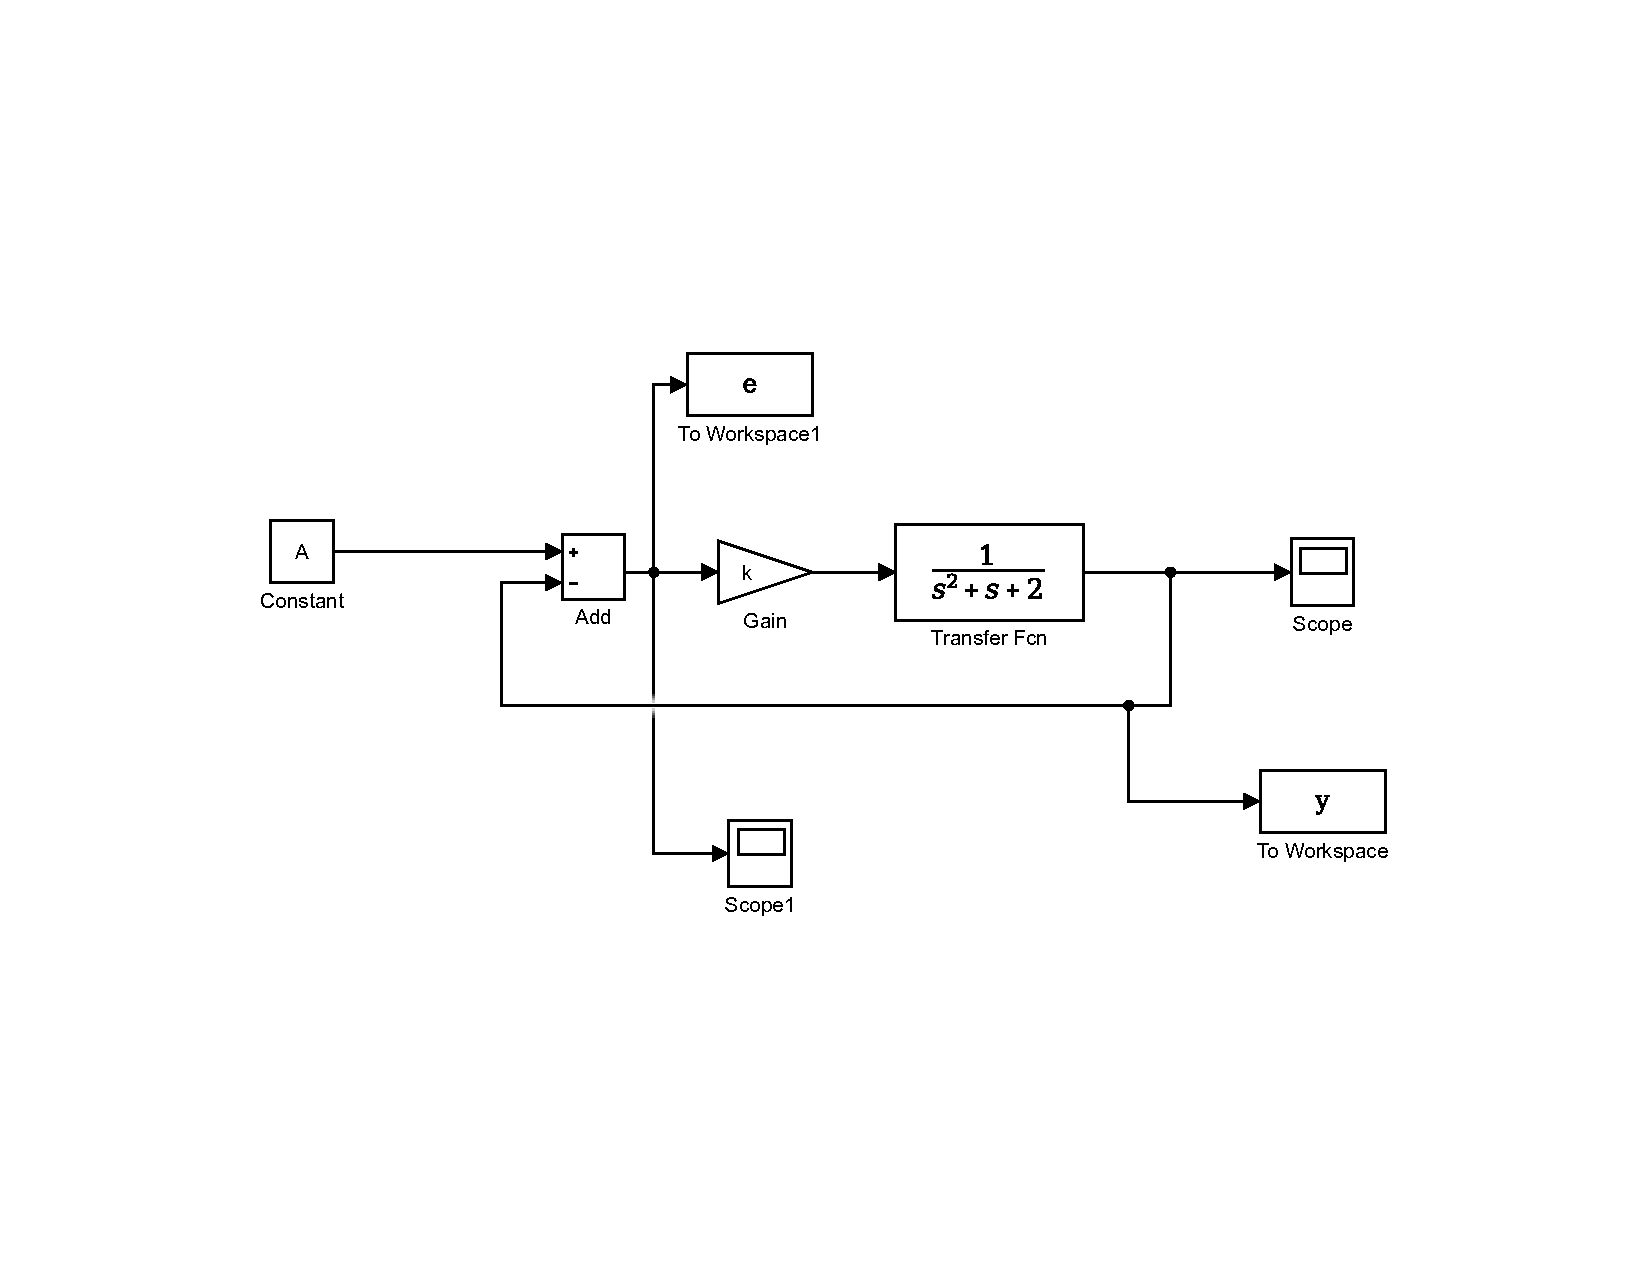
\includegraphics[width=6in]{Astatism00MOD.pdf}
		\caption{Схема моделирования}
		\label{s_1}
	\end{figure}
	\newpage 
	\paragraph {}Переходные процессы и график ошибки при различных значениях $k$ представлены на рисунках \ref{s_2} и \ref{s_3} соответственно

	\begin{figure}[h!]
			\begin{center}
		\renewcommand{\figurename}{Рисунок}
		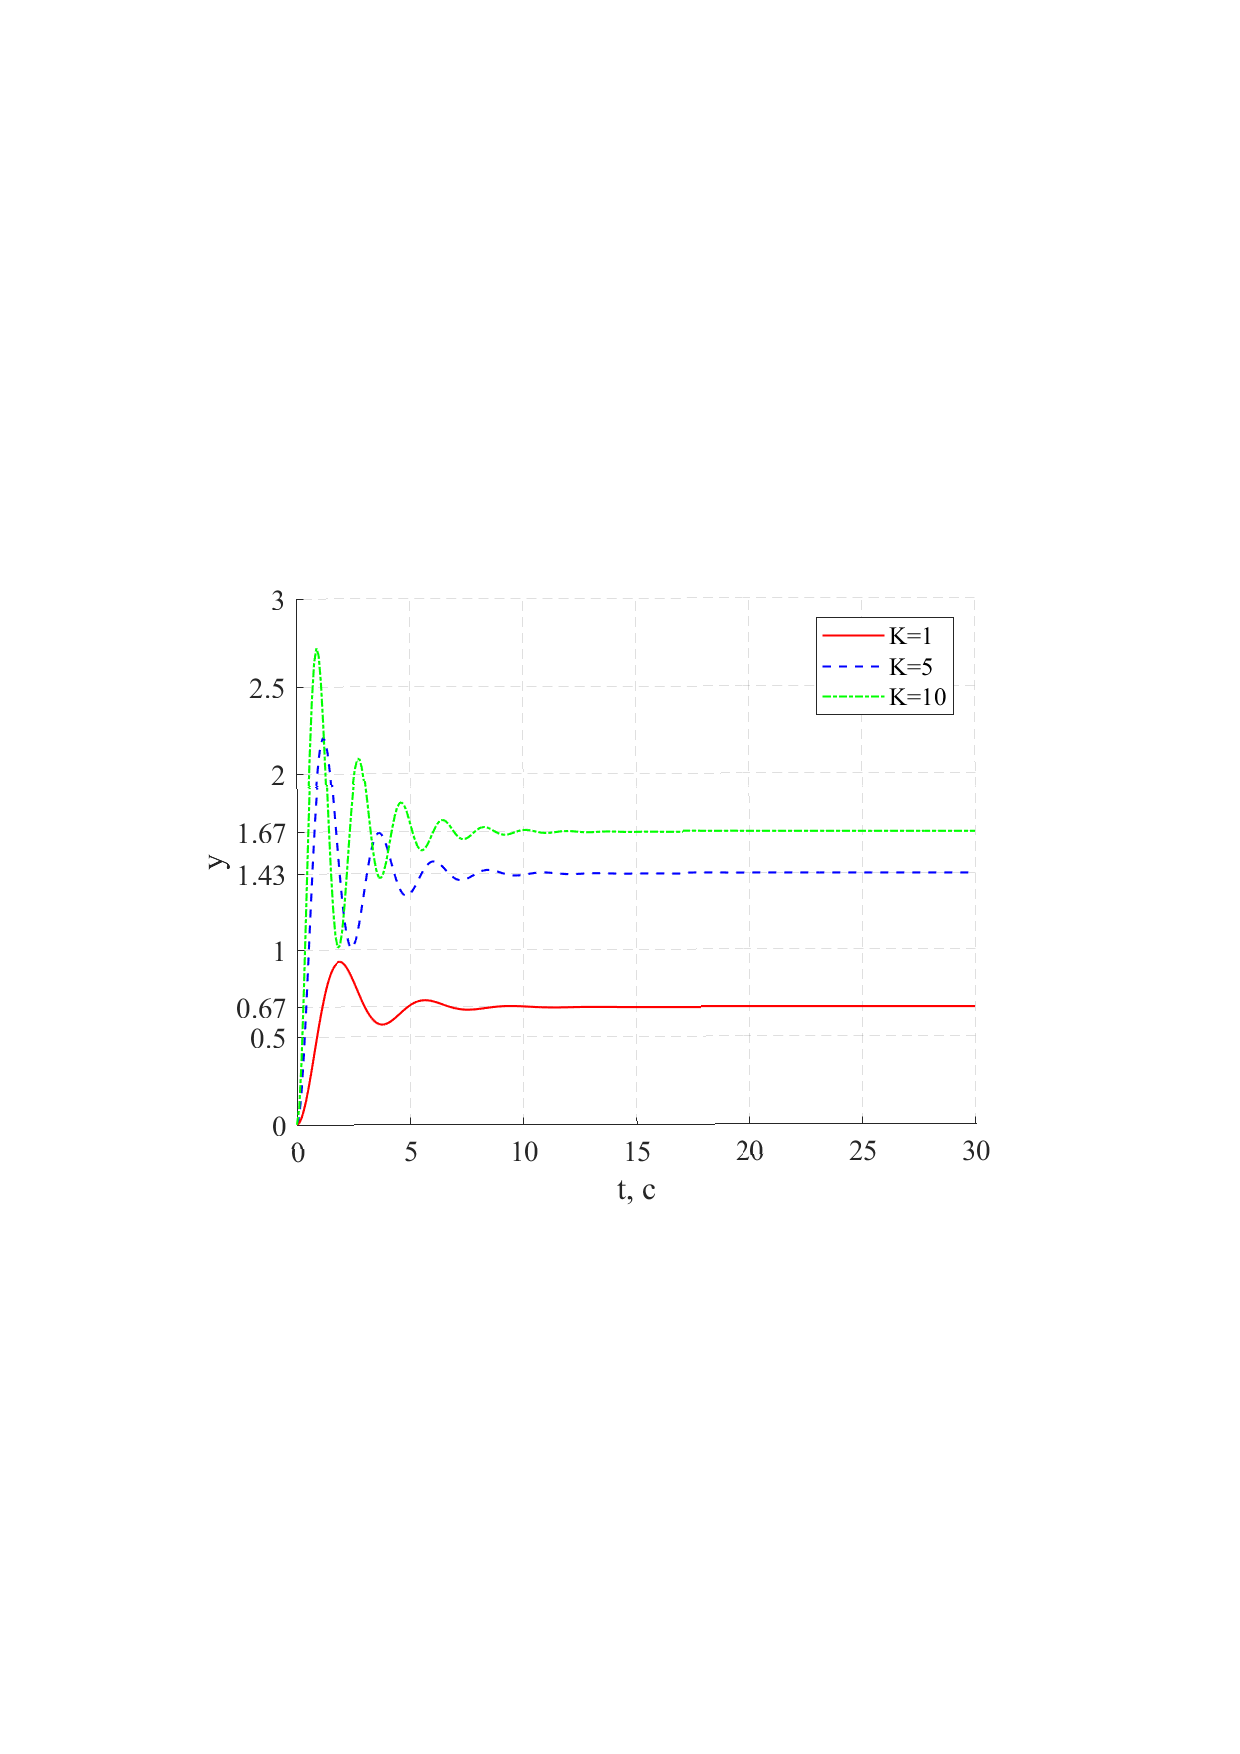
\includegraphics[width=5in]{ph1MOD.pdf}
		\caption{Переходные процессы} 
		\label{s_2} 
		\end{center}
	\end{figure}		
	\begin{figure}[h!]
		\begin{center}
		\renewcommand{\figurename}{Рисунок}
		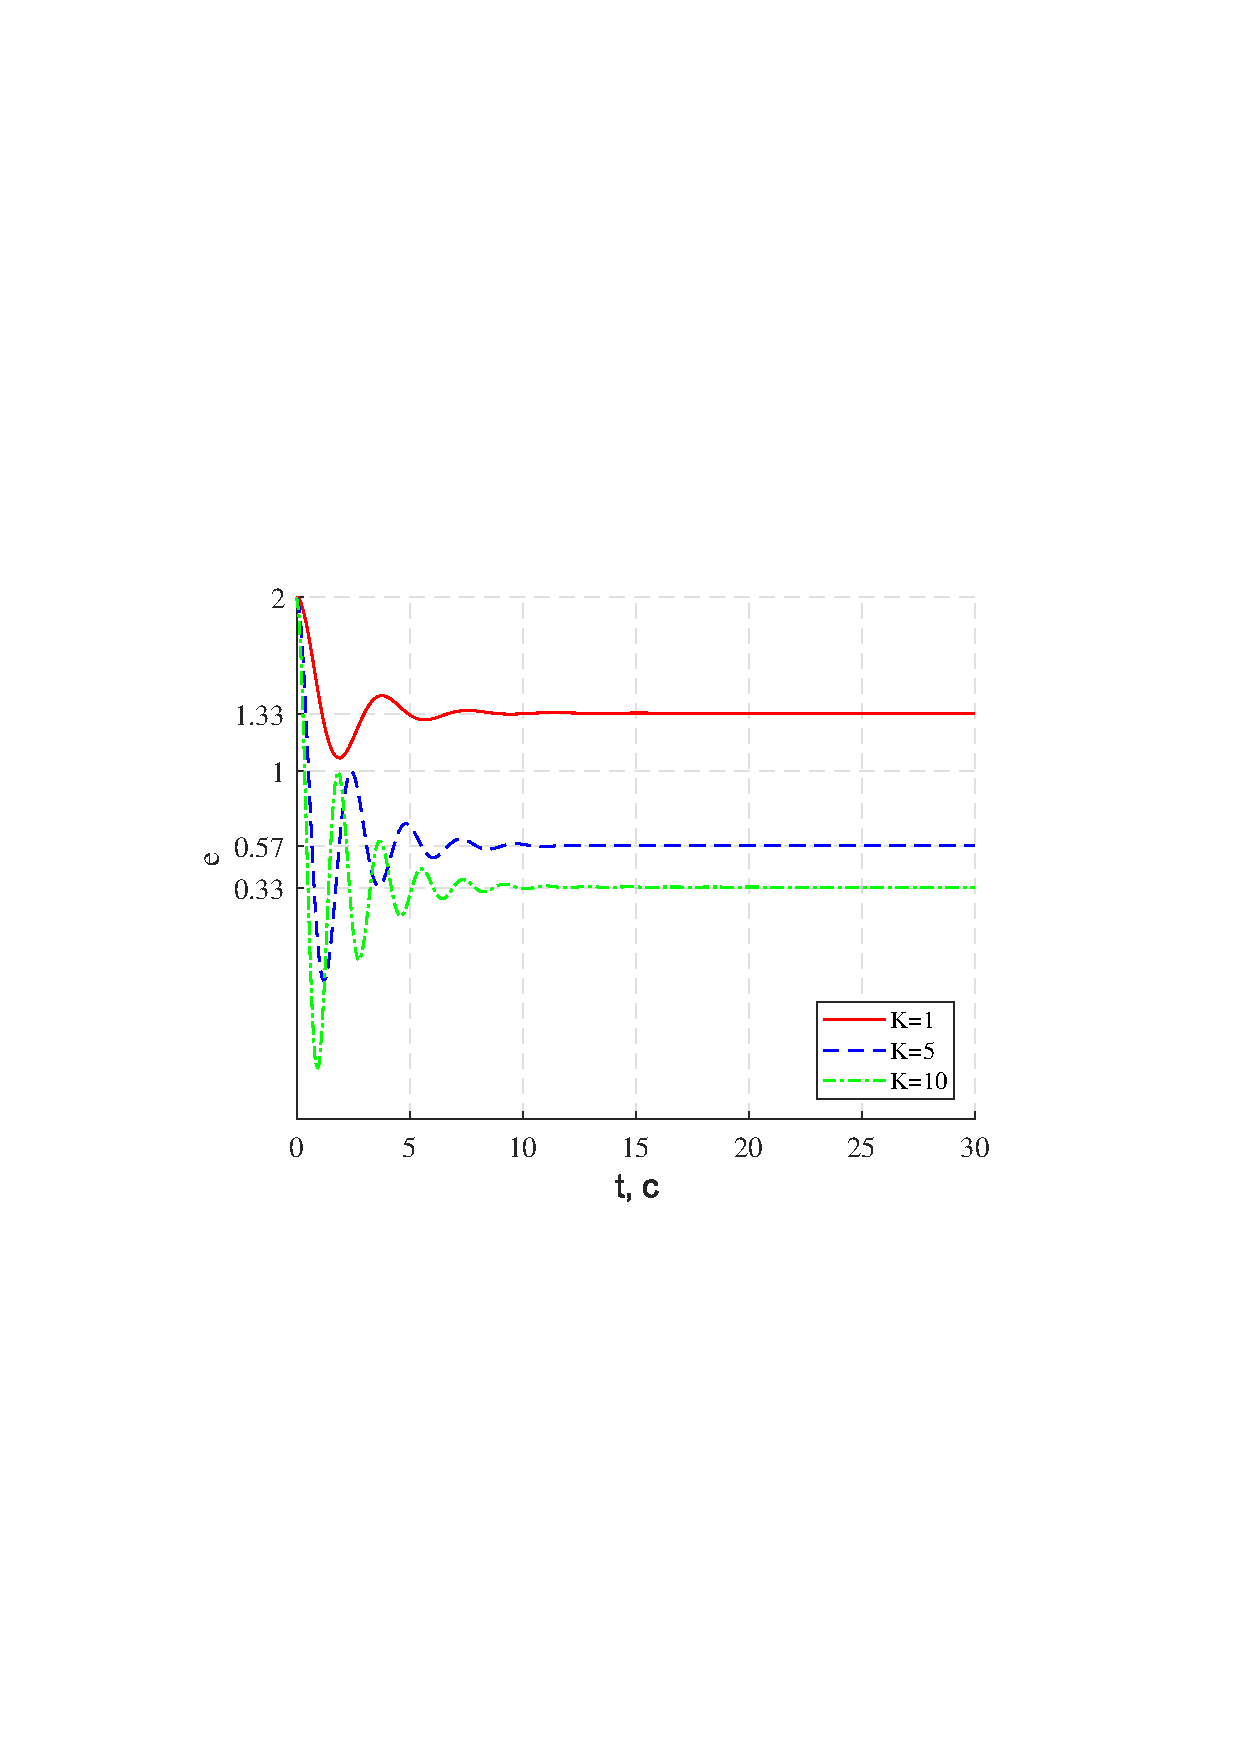
\includegraphics[width=5in]{err1MOD.pdf}
		\caption{Ошибка}
		\label{s_3}
	\end{center}
	\end{figure}
	
	\newpage
	\paragraph {} Аналитический рассчет установившейся ошибки:\\
	\begin{gather}
	\varepsilon=\lim\limits_{s\rightarrow 0}\frac{A}{1+kW(s)}=\lim\limits_{s\rightarrow 0}\frac{2(s^2+s+2)}{s^2+s+2+k}
	\end{gather}
	\begin{itemize}
		\item При $k=1$ ~~:~ $\varepsilon=1.33$
		\item При $k=5$ ~~:~ $\varepsilon=0.57$
		\item При $k=10$~:~ $\varepsilon=0.33$
	\end{itemize}
	\subsection{Исследование режима движения с постоянной скоростью:\\ $g(t)=Vt$}
	\paragraph {} Схема моделирования представлена на рисунке \ref{s_4}
	
	\begin{figure}[h]
		\renewcommand{\figurename}{Рисунок}
		\centering
		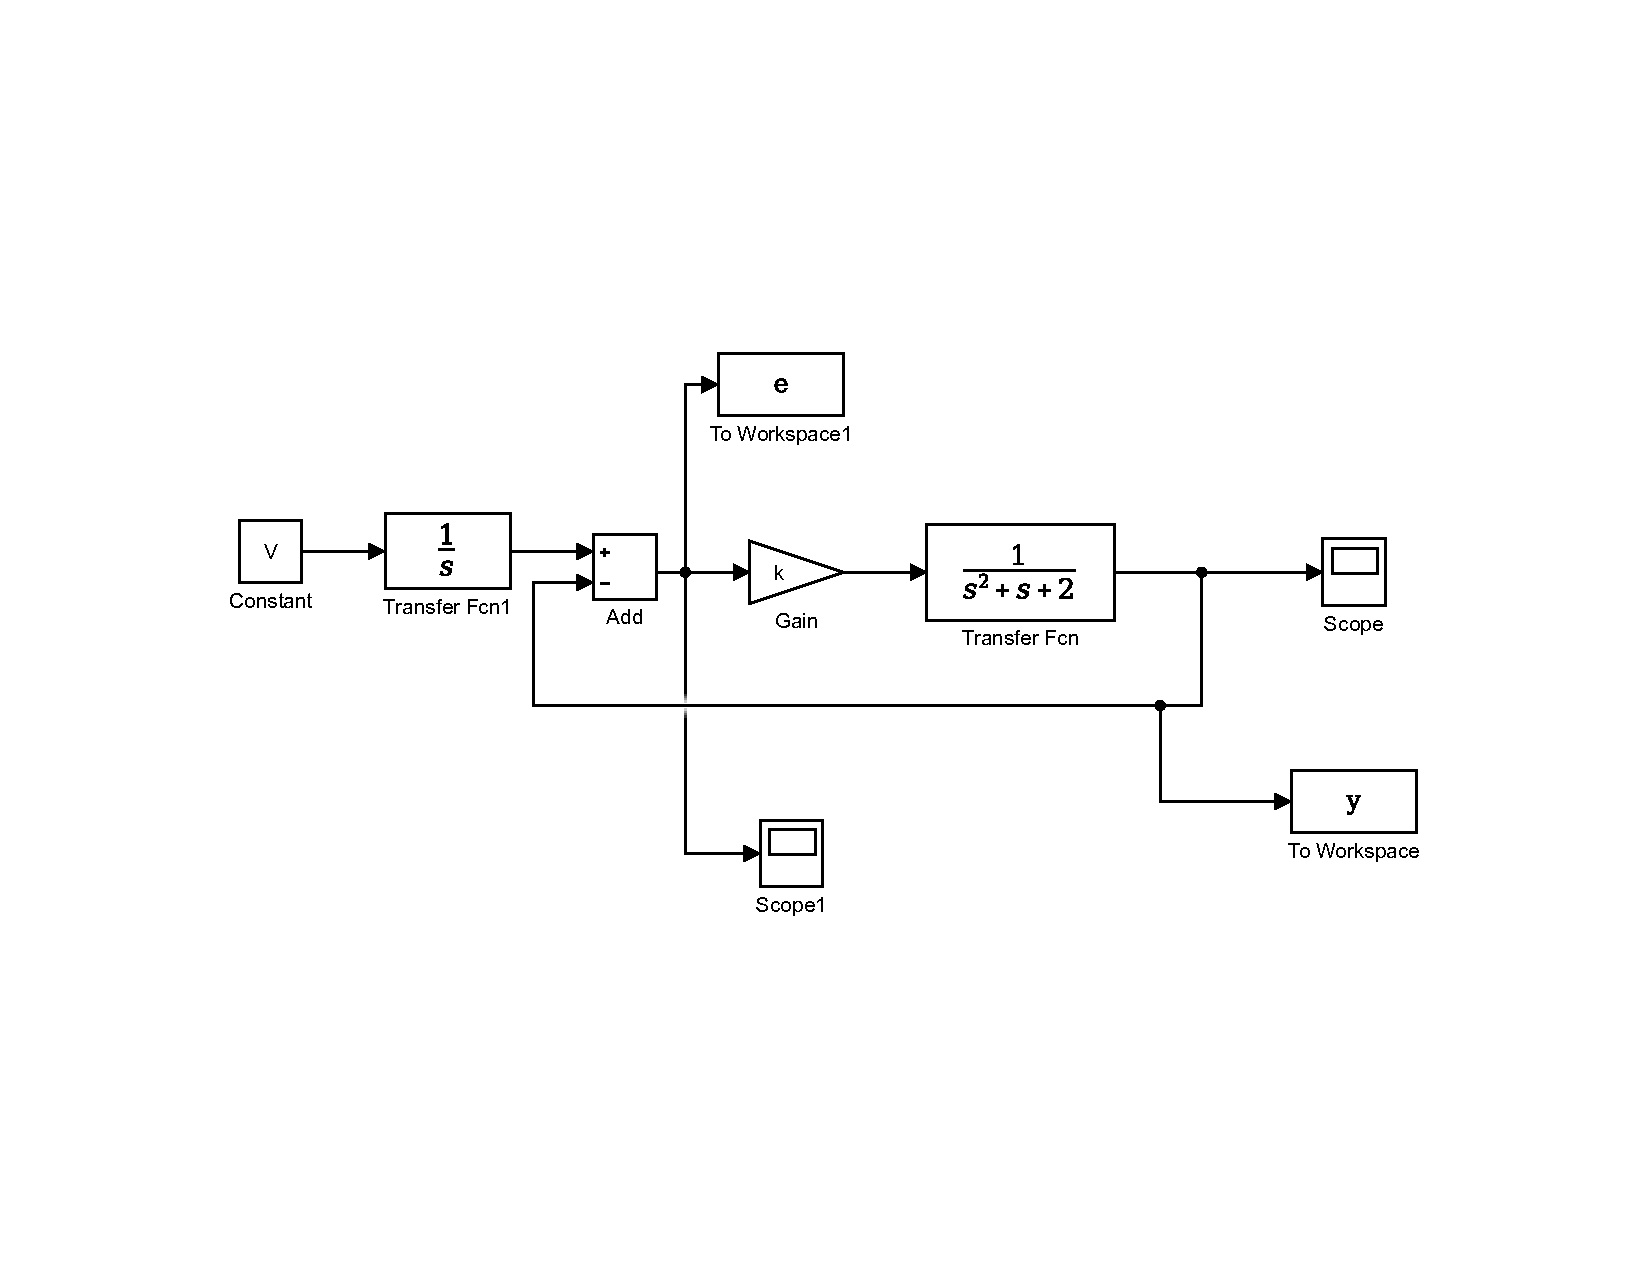
\includegraphics[width=6in]{Astatism0VMOD.pdf}
		\caption{Схема моделирования}
		\label{s_4}
	\end{figure}
	\newpage 
	\paragraph {}Переходные процессы и график ошибки при различных значениях $k$ представлены на рисунках \ref{s_5} и \ref{s_6} соответственно
	
	\begin{figure}[h!]
		\begin{center}
		\renewcommand{\figurename}{Рисунок}
		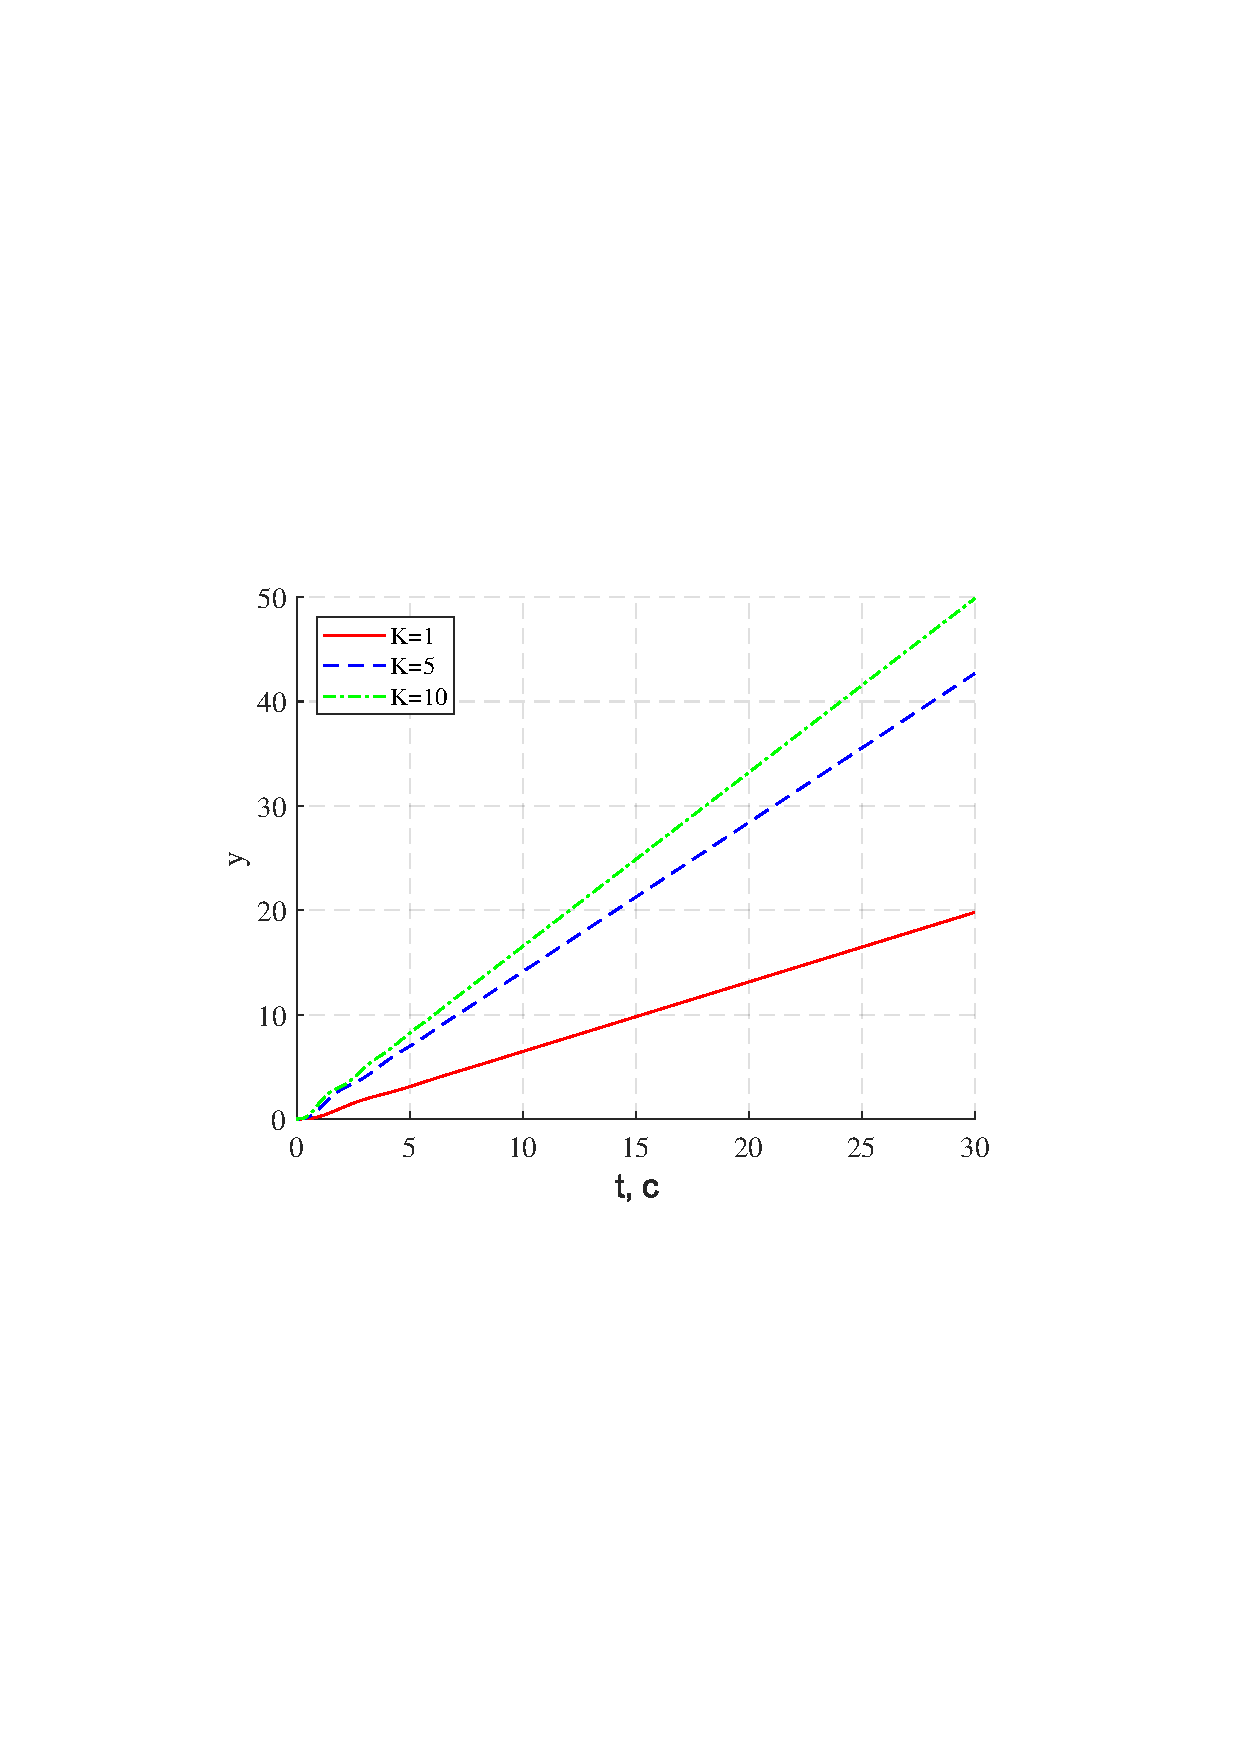
\includegraphics[width=5in]{ph2MOD.pdf}
		\caption{Переходные процессы} 
		\label{s_5}
		\end{center} 
	\end{figure}
	\begin{figure}[h!]
		\begin{center}
		\renewcommand{\figurename}{Рисунок}
		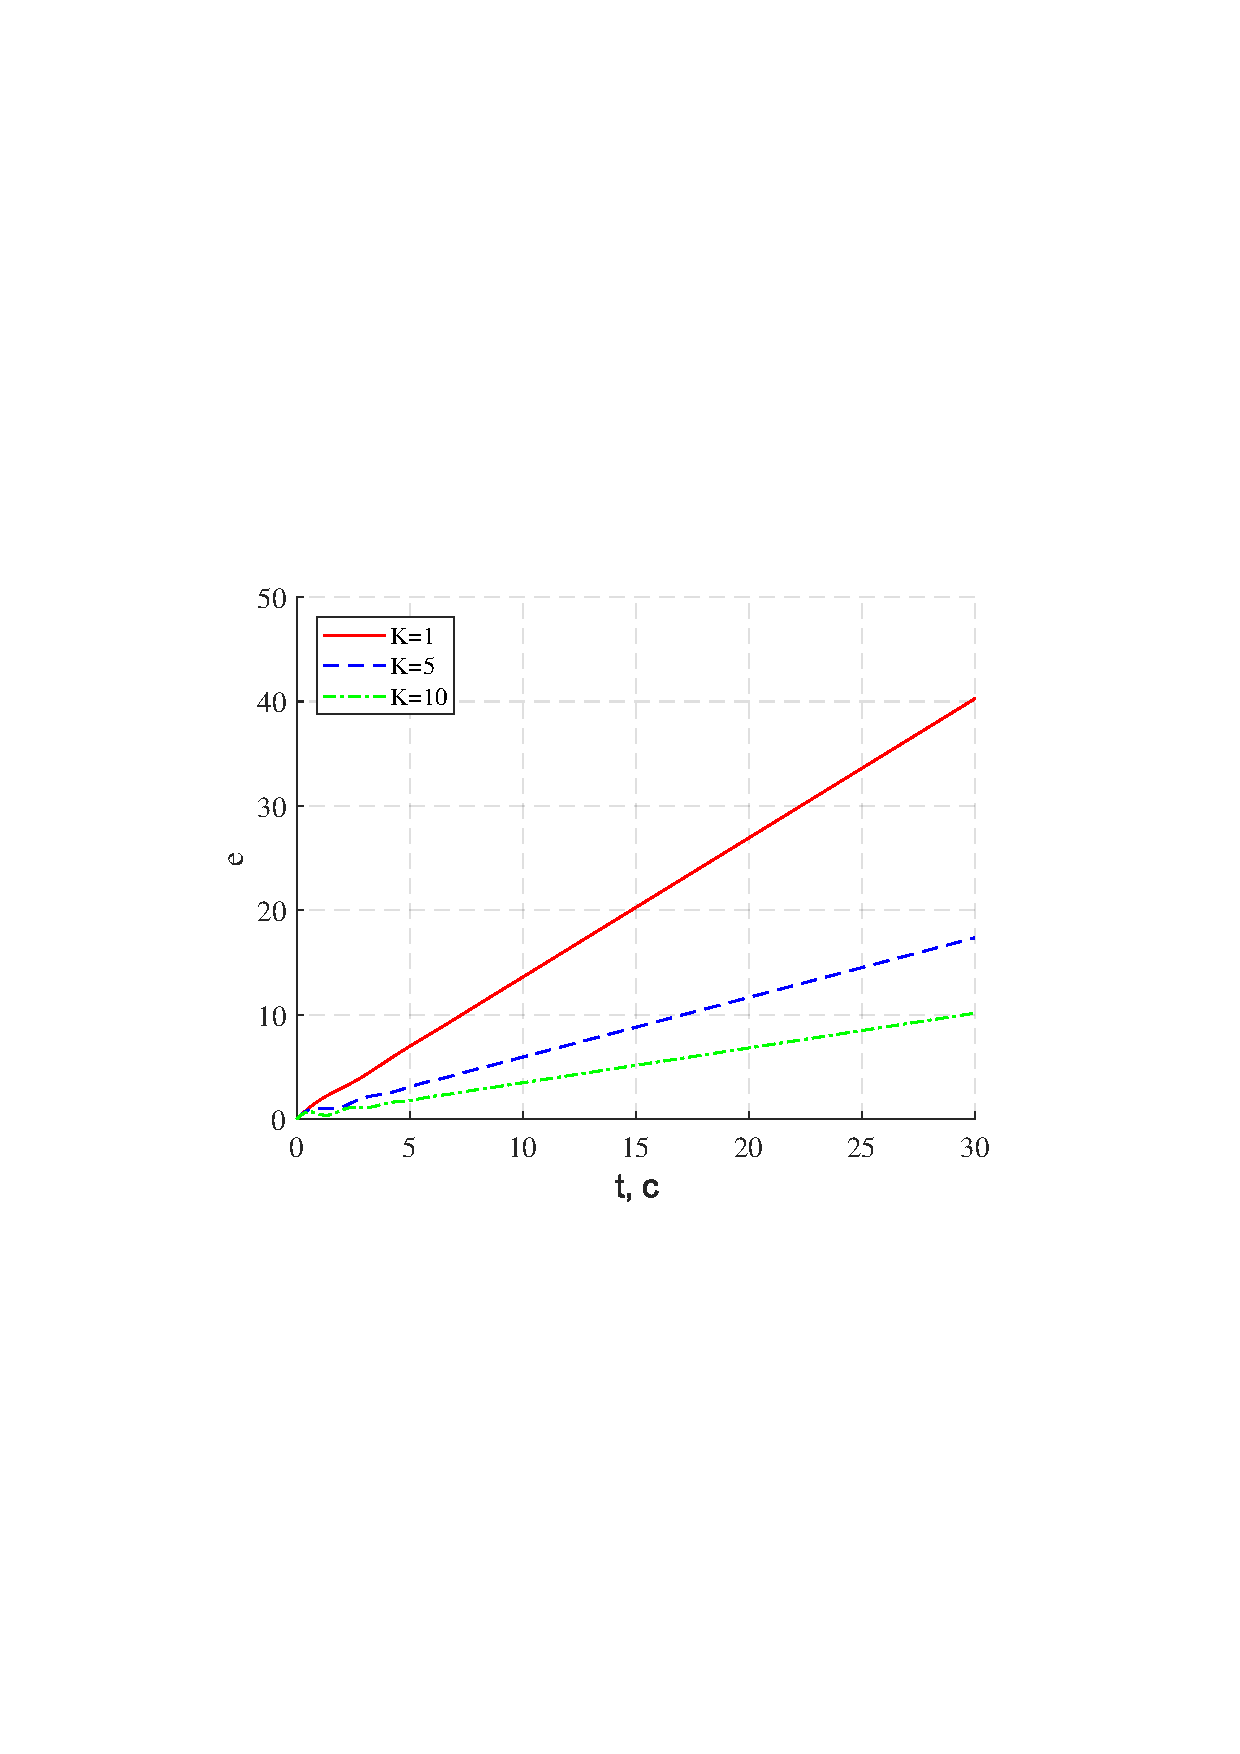
\includegraphics[width=5in]{err2MOD.pdf}
		\caption{Ошибка}
		\label{s_6}
		\end{center}	
	\end{figure}
	
	\newpage
	
	\begin{center}
		\section{Исследование системы с астатизмом первого порядка}
	\end{center}
	
	\subsection{Исследование стационарного режима работы: $g(t)=A$}
	\paragraph {} Схема моделирования представлена на рисунке \ref{s_7}
	
	\begin{figure}[h]
		\renewcommand{\figurename}{Рисунок}
		\centering
		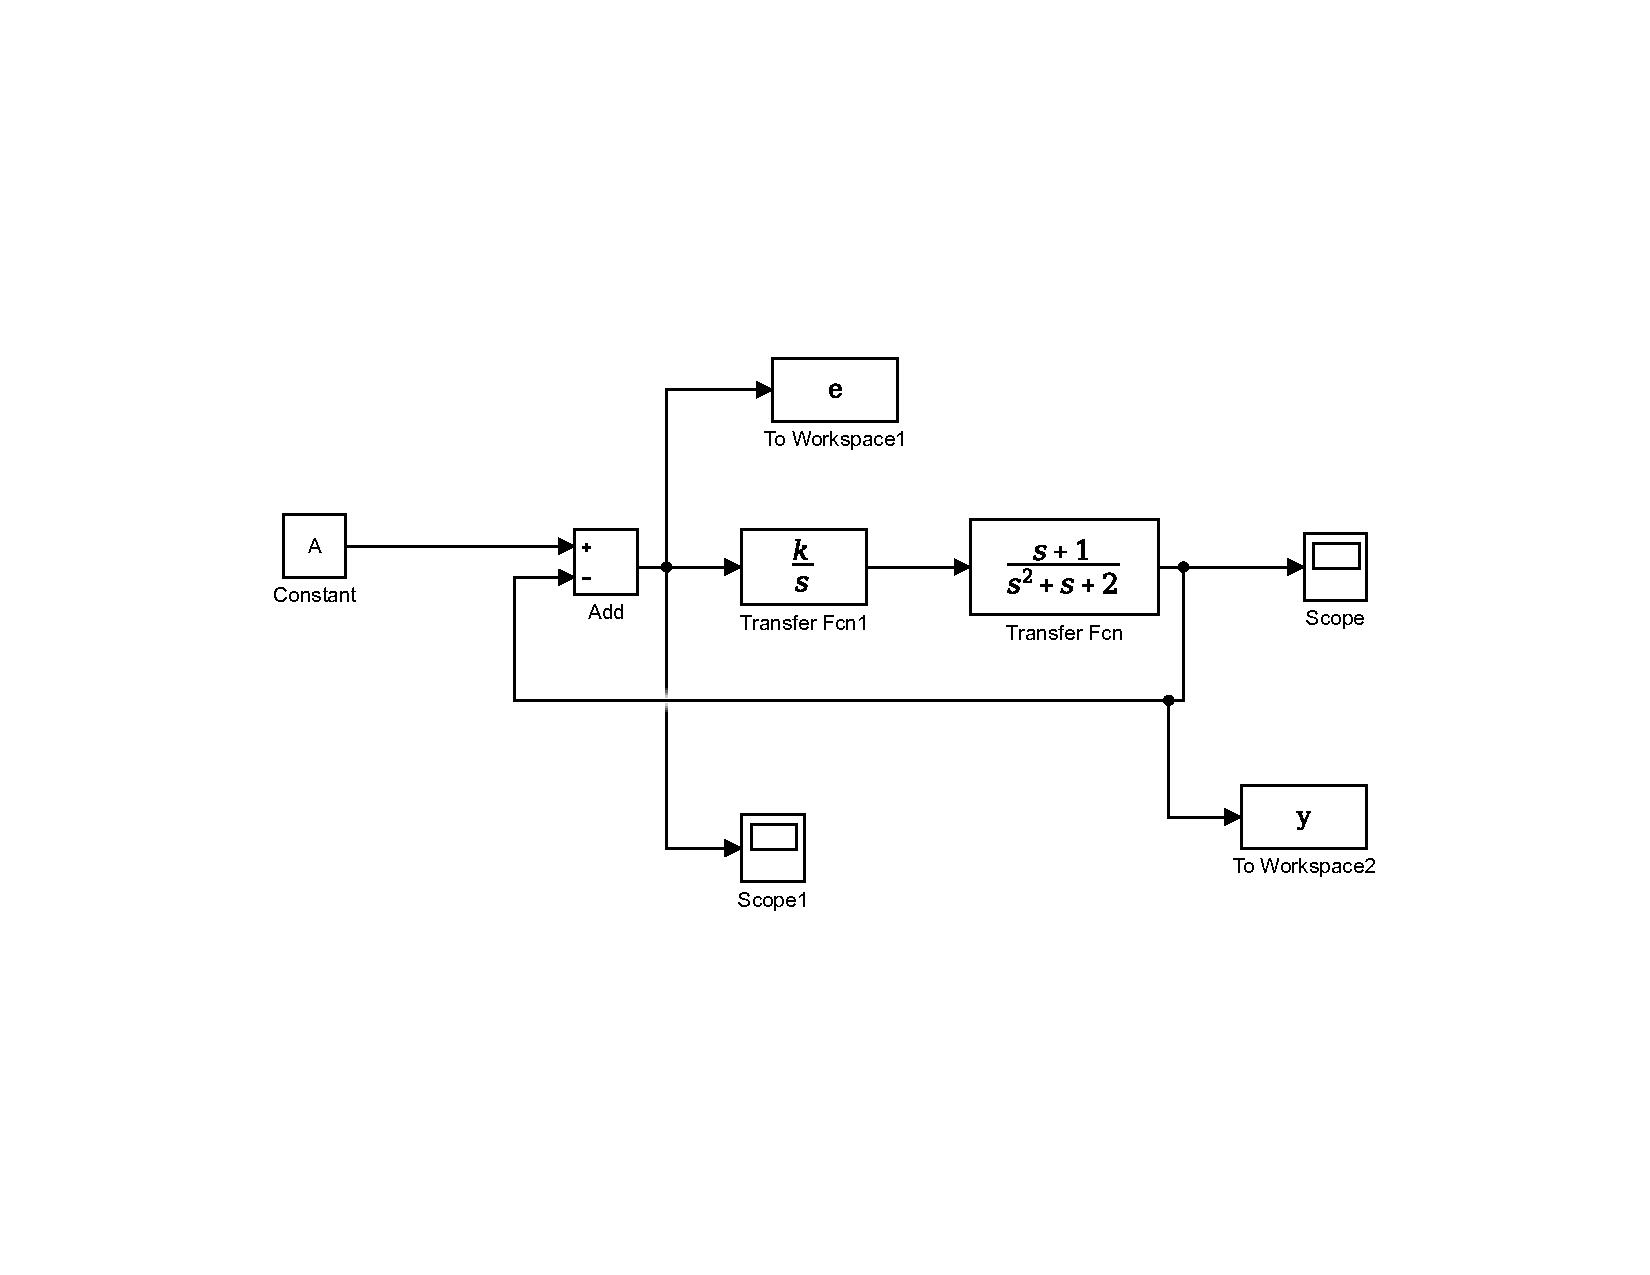
\includegraphics[width=6in]{Astatizm10MOD.pdf}
		\caption{Схема моделирования}
		\label{s_7}
	\end{figure}
	\newpage
	\paragraph {}Переходные процессы и график ошибки при различных значениях $k$ представлены на рисунках \ref{s_8} и \ref{s_9} соответственно
	
	\begin{figure}[h!]
		\begin{center}
		\renewcommand{\figurename}{Рисунок}
		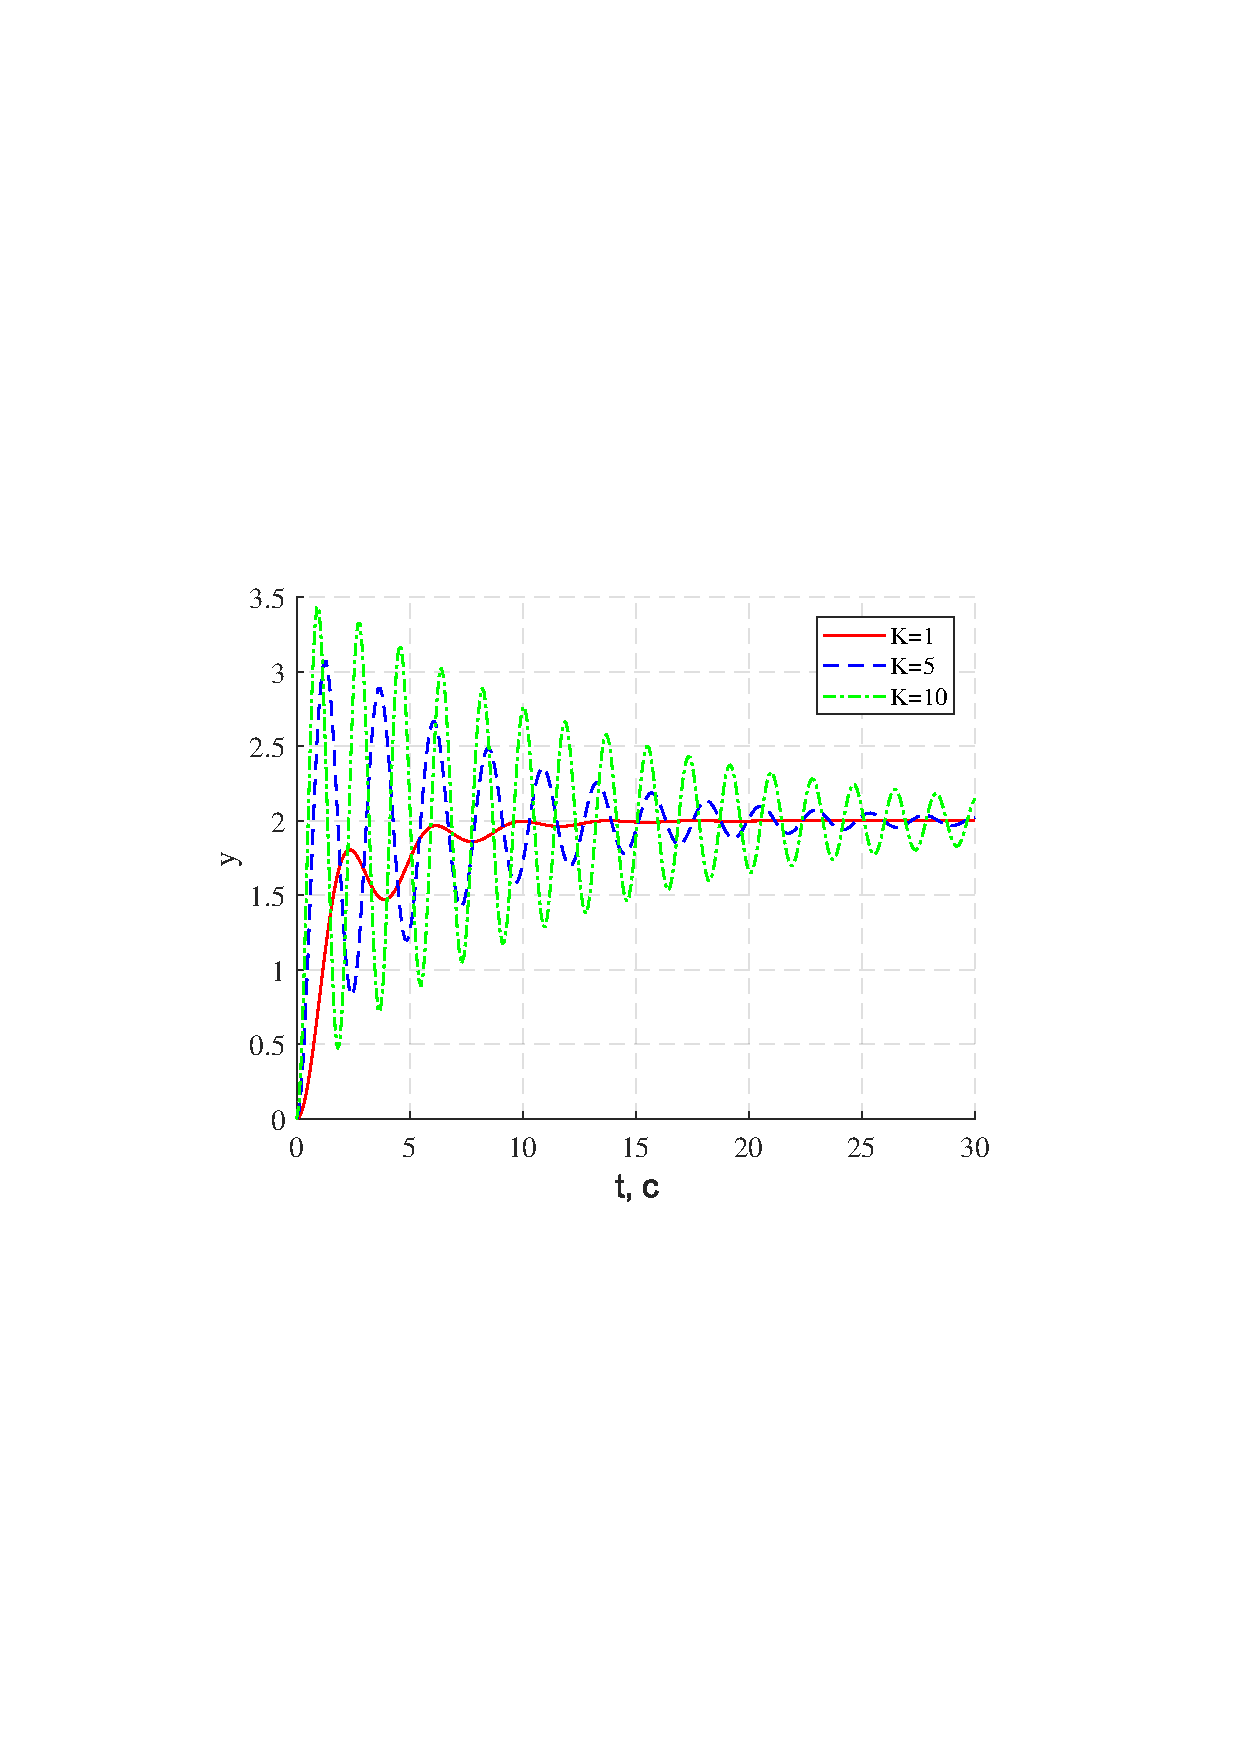
\includegraphics[width=5in]{ph1ast1MOD.pdf}
		\caption{Переходные процессы} 
		\label{s_8}
		\end{center}
	\end{figure} 
	\begin{figure}[h!]
		\begin{center}
		\renewcommand{\figurename}{Рисунок}
		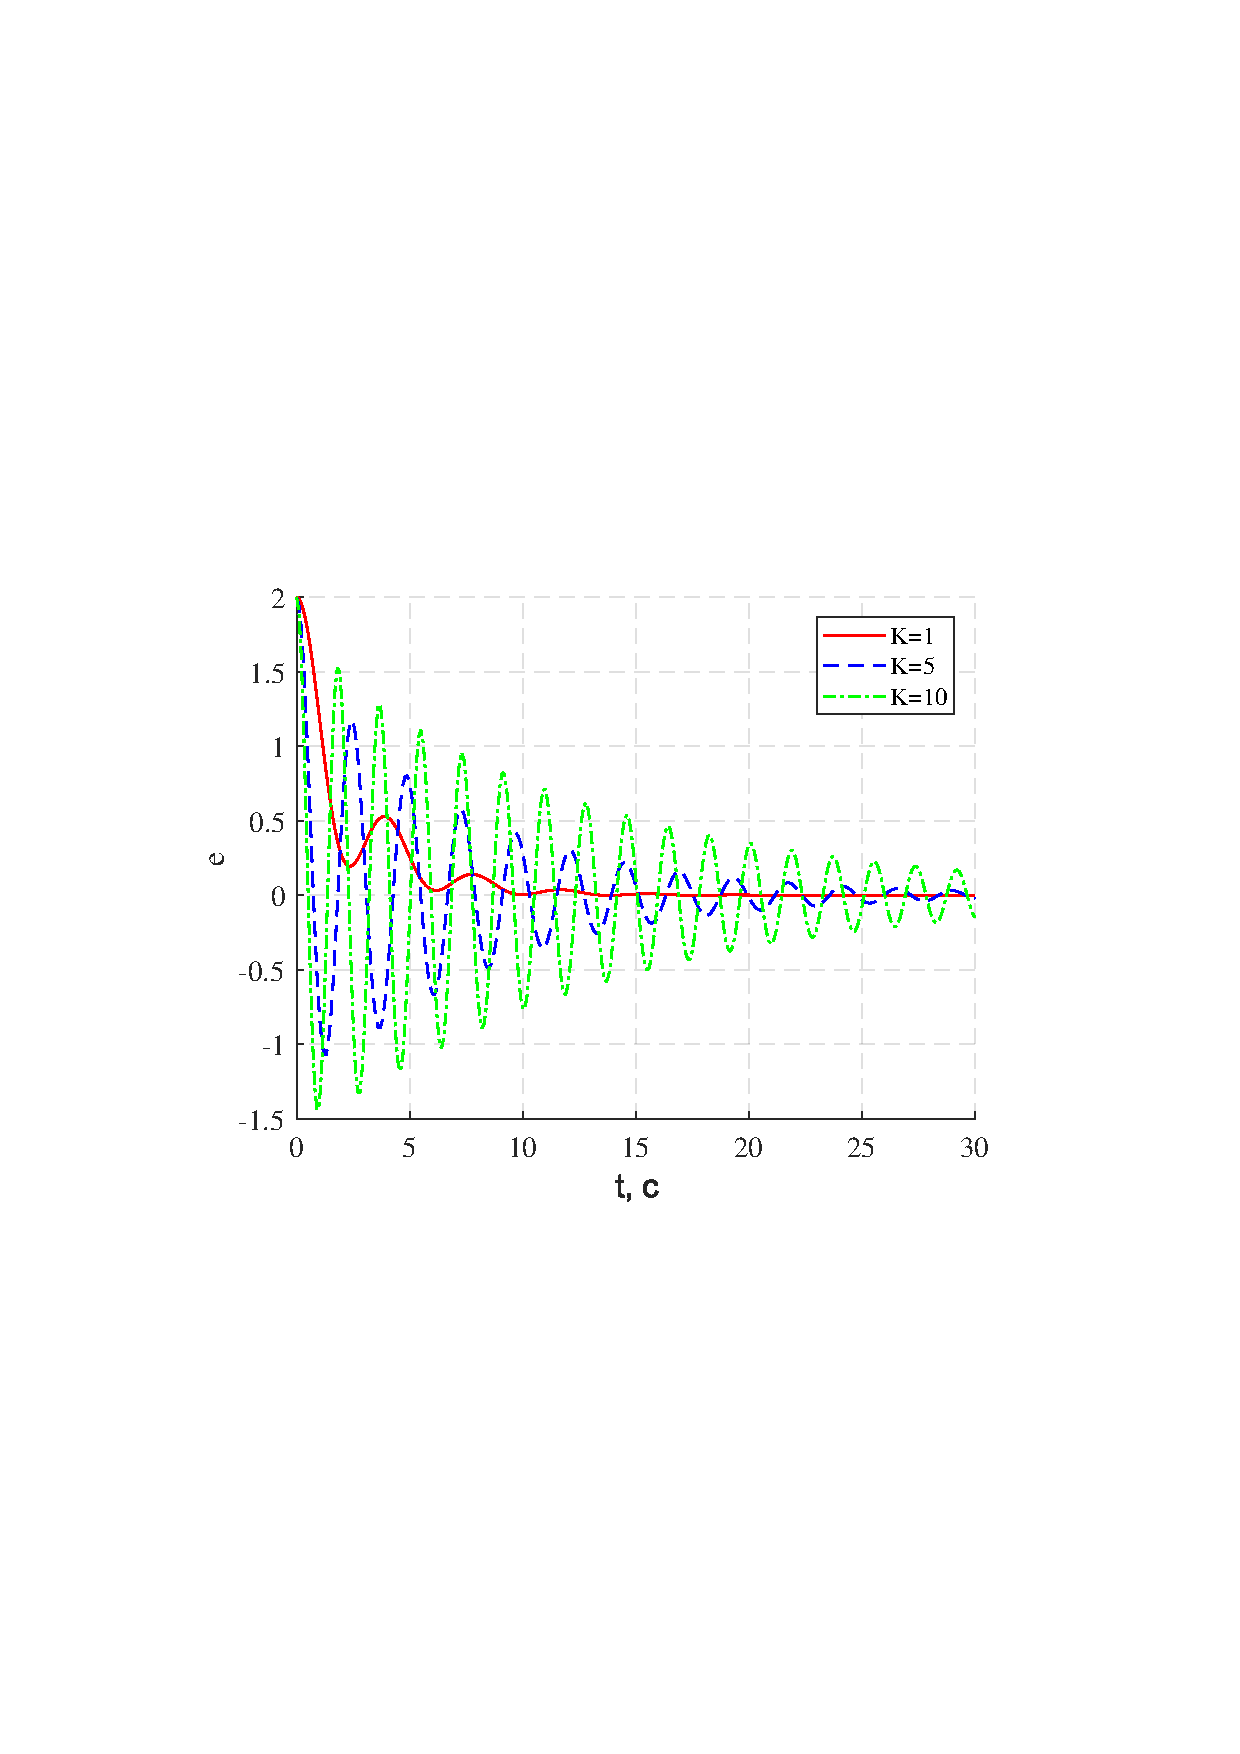
\includegraphics[width=5in]{err1ast1MOD.pdf}
		\caption{Ошибка}
		\label{s_9}
		\end{center}
	\end{figure}
	\newpage
	\paragraph {} Аналитический рассчет установившейся ошибки:\\
	\begin{gather}
	\varepsilon=\lim\limits_{s\rightarrow 0}s\frac{A}{1+kW(s)}=\lim\limits_{s\rightarrow 0}s\frac{2(s^2+s+2)}{s^2+s+2+k}=0
	\end{gather}
	
	\subsection{Исследование режима движения с постоянной скоростью:\\ $g(t)=Vt$}
	\paragraph {} Схема моделирования представлена на рисунке \ref{s_10}
	
	\begin{figure}[h]
		\renewcommand{\figurename}{Рисунок}
		\centering
		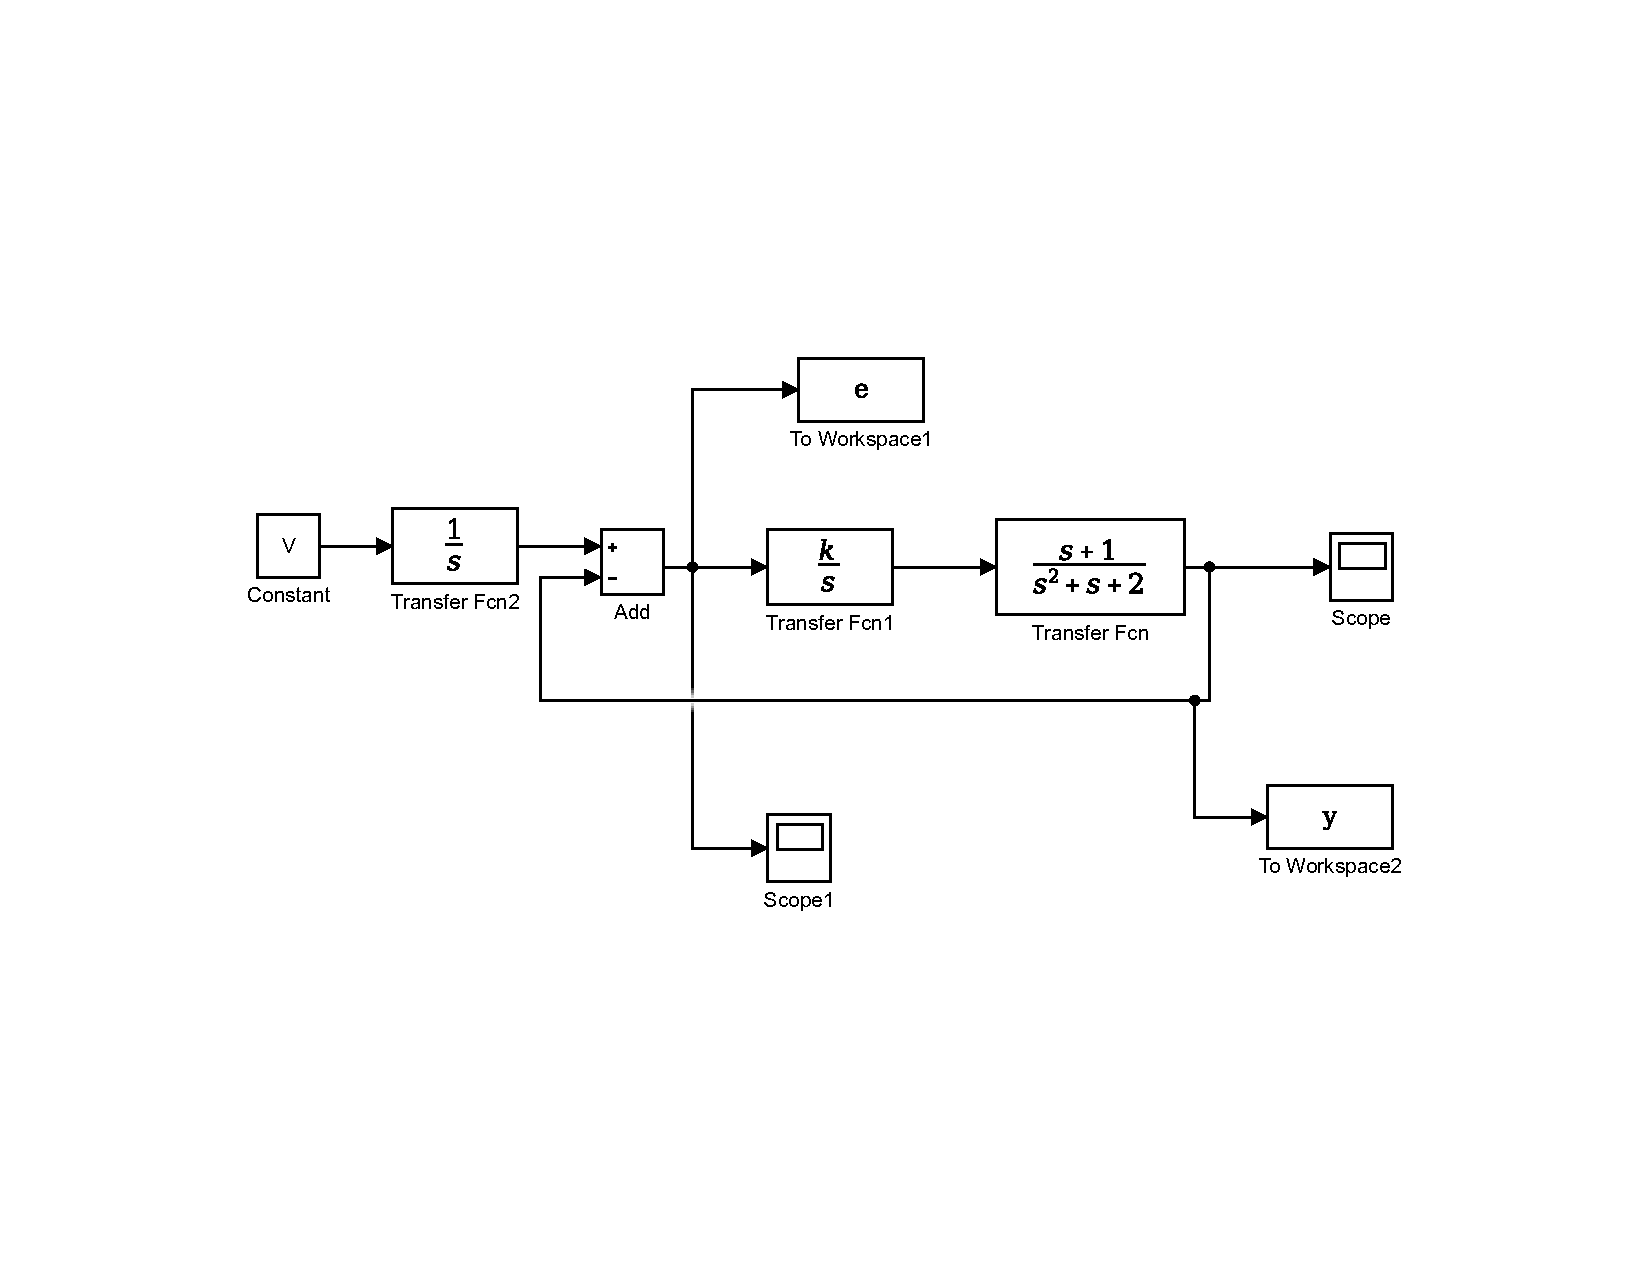
\includegraphics[width=6in]{Astatizm1VMOD.pdf}
		\caption{Схема моделирования}
		\label{s_10}
	\end{figure}
	\newpage 
	\paragraph {}Переходные процессы и график ошибки при различных значениях $k$ представлены на рисунках \ref{s_11} и \ref{s_12} соответственно
	
	\begin{figure}[h!]
		\begin{center}
		\renewcommand{\figurename}{Рисунок}
		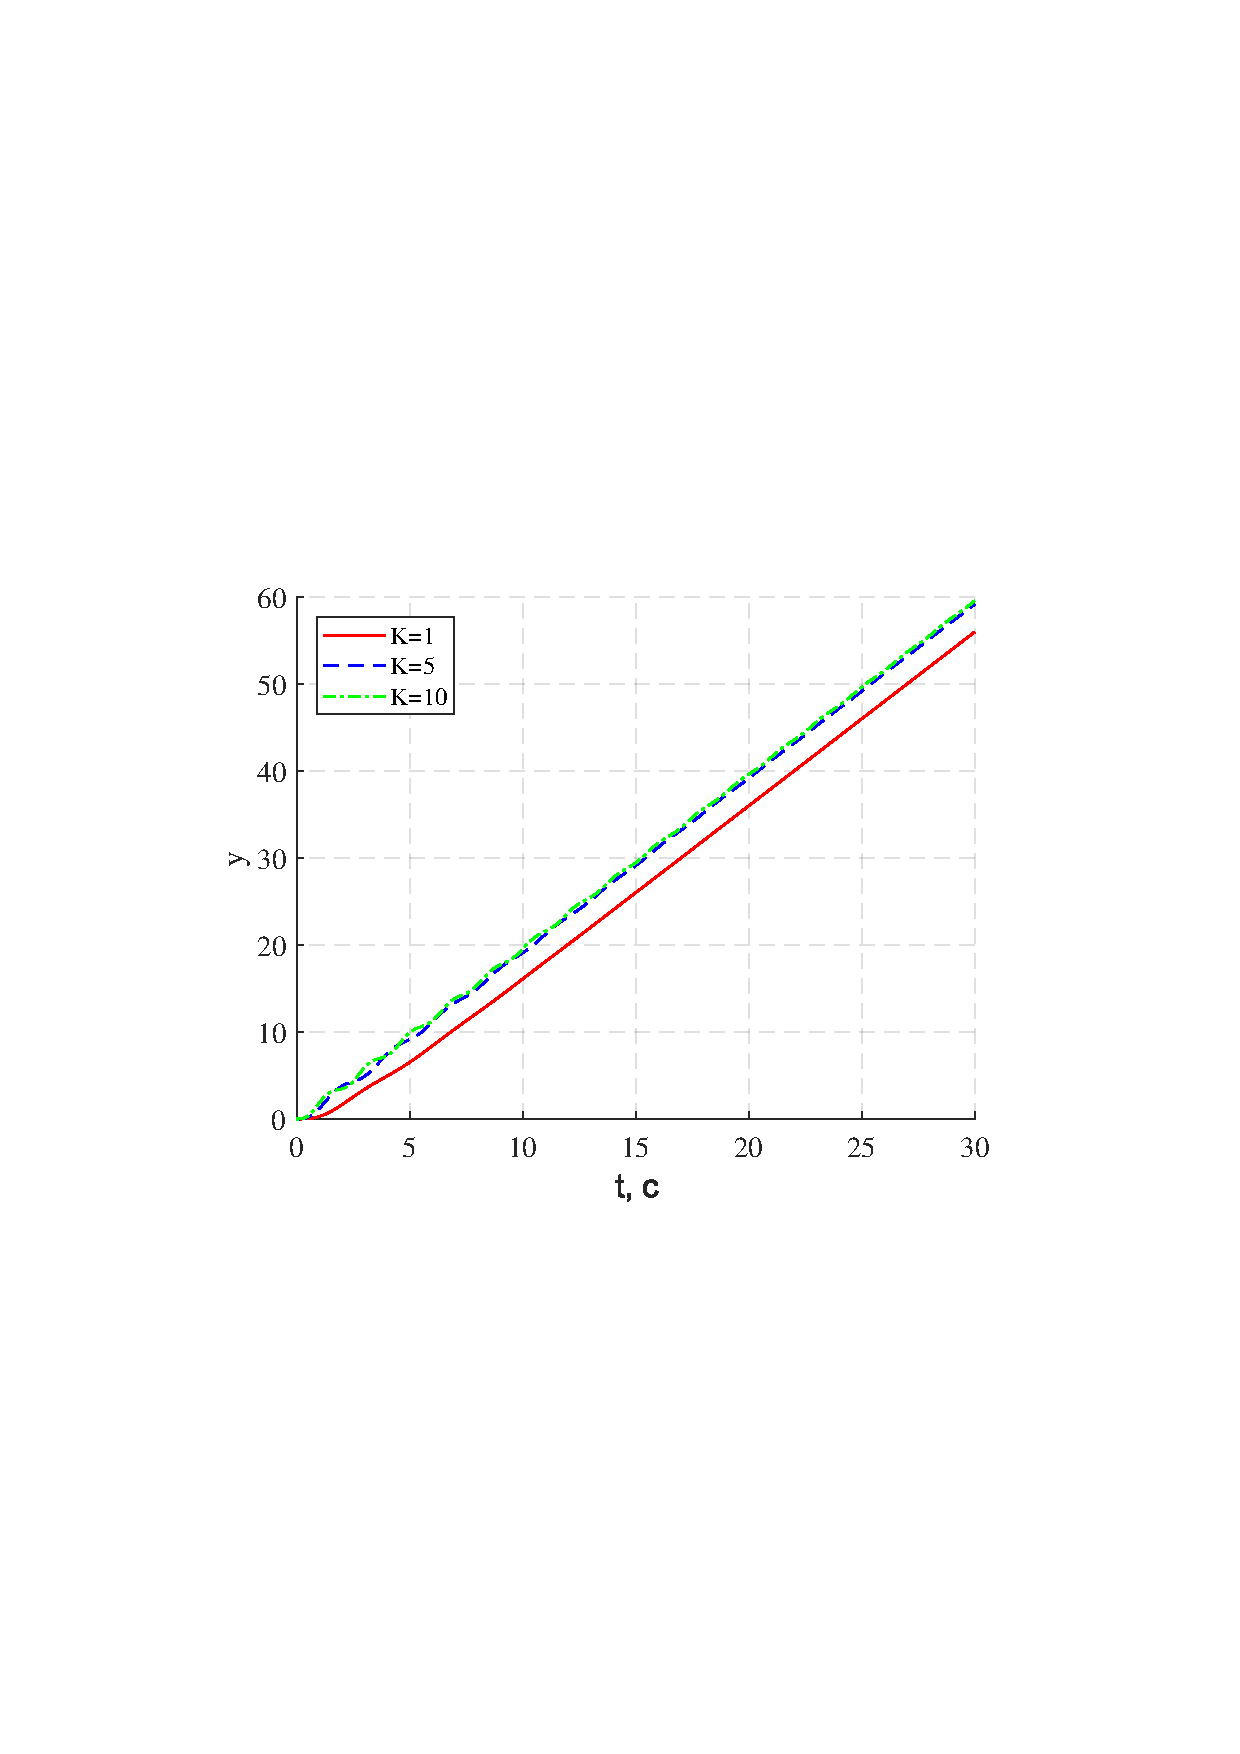
\includegraphics[width=5in]{ph2ast1MOD.pdf}
		\caption{Переходные процессы} 
		\label{s_11} 
		\end{center}
	\end{figure}
	\begin{figure}[h!]
		\begin{center}			
		\renewcommand{\figurename}{Рисунок}
		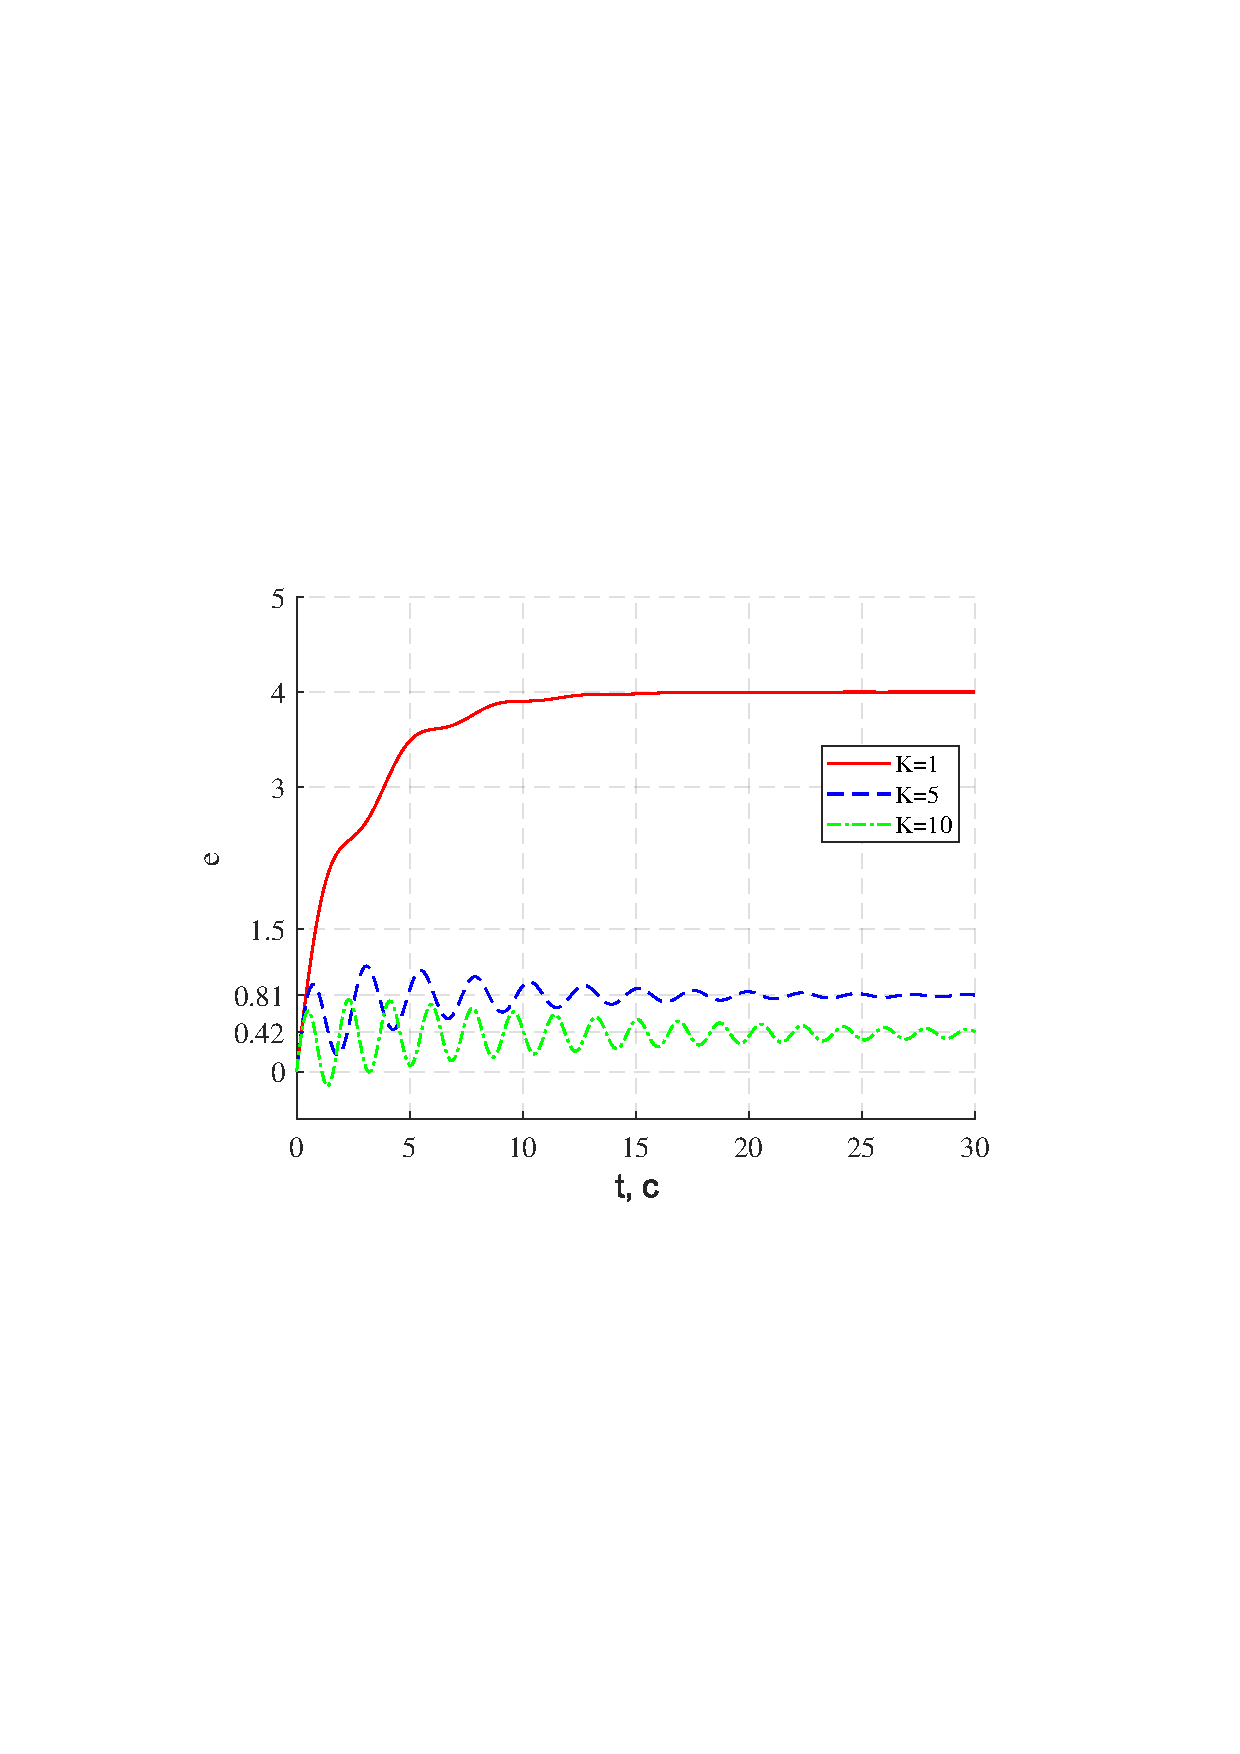
\includegraphics[width=5in]{err2ast1MOD.pdf}
		\caption{Ошибка}
		\label{s_12}
		\end{center}
	\end{figure}
	\newpage		
	\paragraph {} Аналитический рассчет установившейся ошибки:\\
	\begin{gather}
	\varepsilon=\lim\limits_{s\rightarrow 0}\frac{V}{s(1+\frac{k}{s}W(s))}=\lim\limits_{s\rightarrow 0}\frac{V(s^2+s+2)}{s(s^2+s+2+k+\frac{k}{s})}=\frac{2V}{k}
	\end{gather}
	\begin{itemize}
		\item При $k=1$ ~~:~ $\varepsilon=4$
		\item При $k=5$ ~~:~ $\varepsilon=0.8$
		\item При $k=10$~:~ $\varepsilon=0.4$
	\end{itemize}
	\subsection{Исследование режима движения с постоянным ускорением: $g(t)=\frac{at^2}{2}$}
	\paragraph {} Схема моделирования представлена на рисунке \ref{s_13}
	
	\begin{figure}[h]
		\renewcommand{\figurename}{Рисунок}
		\centering
		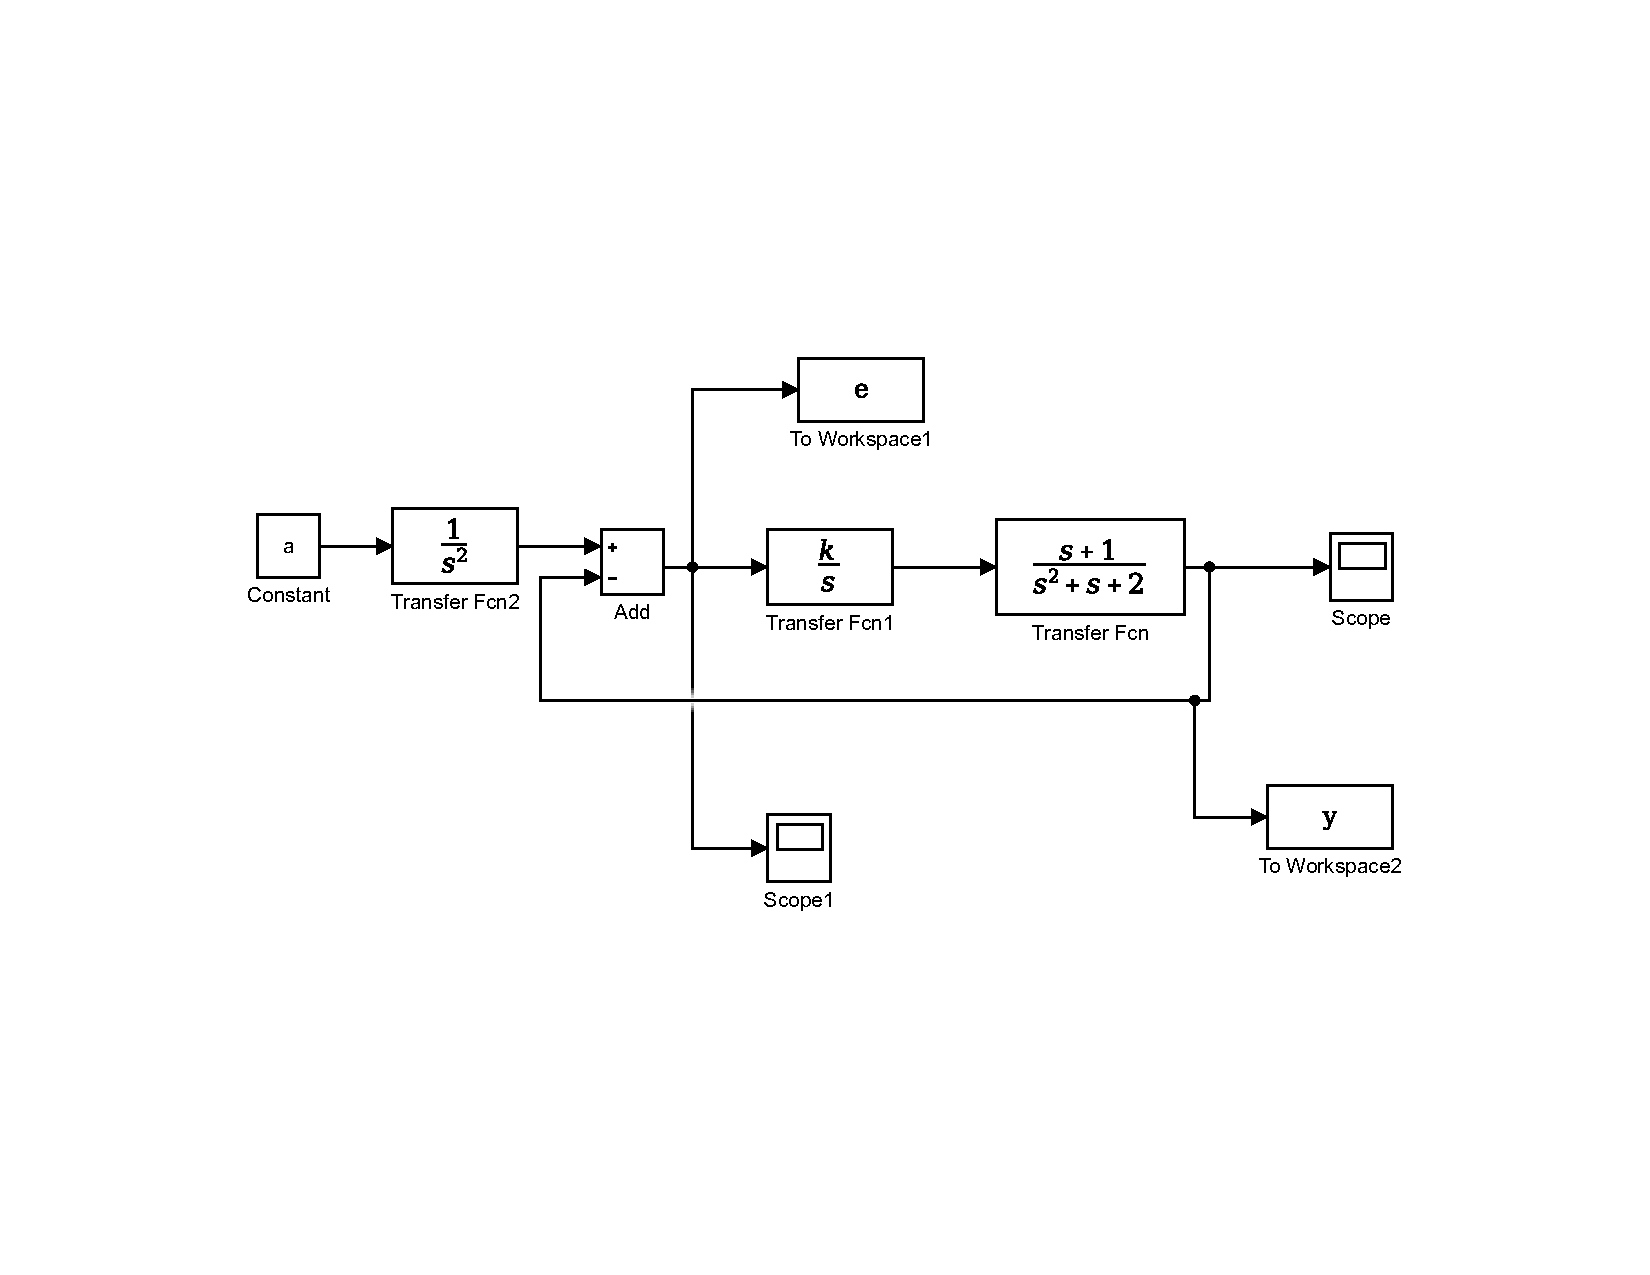
\includegraphics[width=6in]{Astatizm1aMOD.pdf}
		\caption{Схема моделирования}
		\label{s_13}
	\end{figure}
	\newpage 
	\paragraph {}Переходные процессы и график ошибки при различных значениях $k$ представлены на рисунках \ref{s_14} и \ref{s_15} соответственно
	
	\begin{figure}[h!]
		\begin{center}
		\renewcommand{\figurename}{Рисунок}
		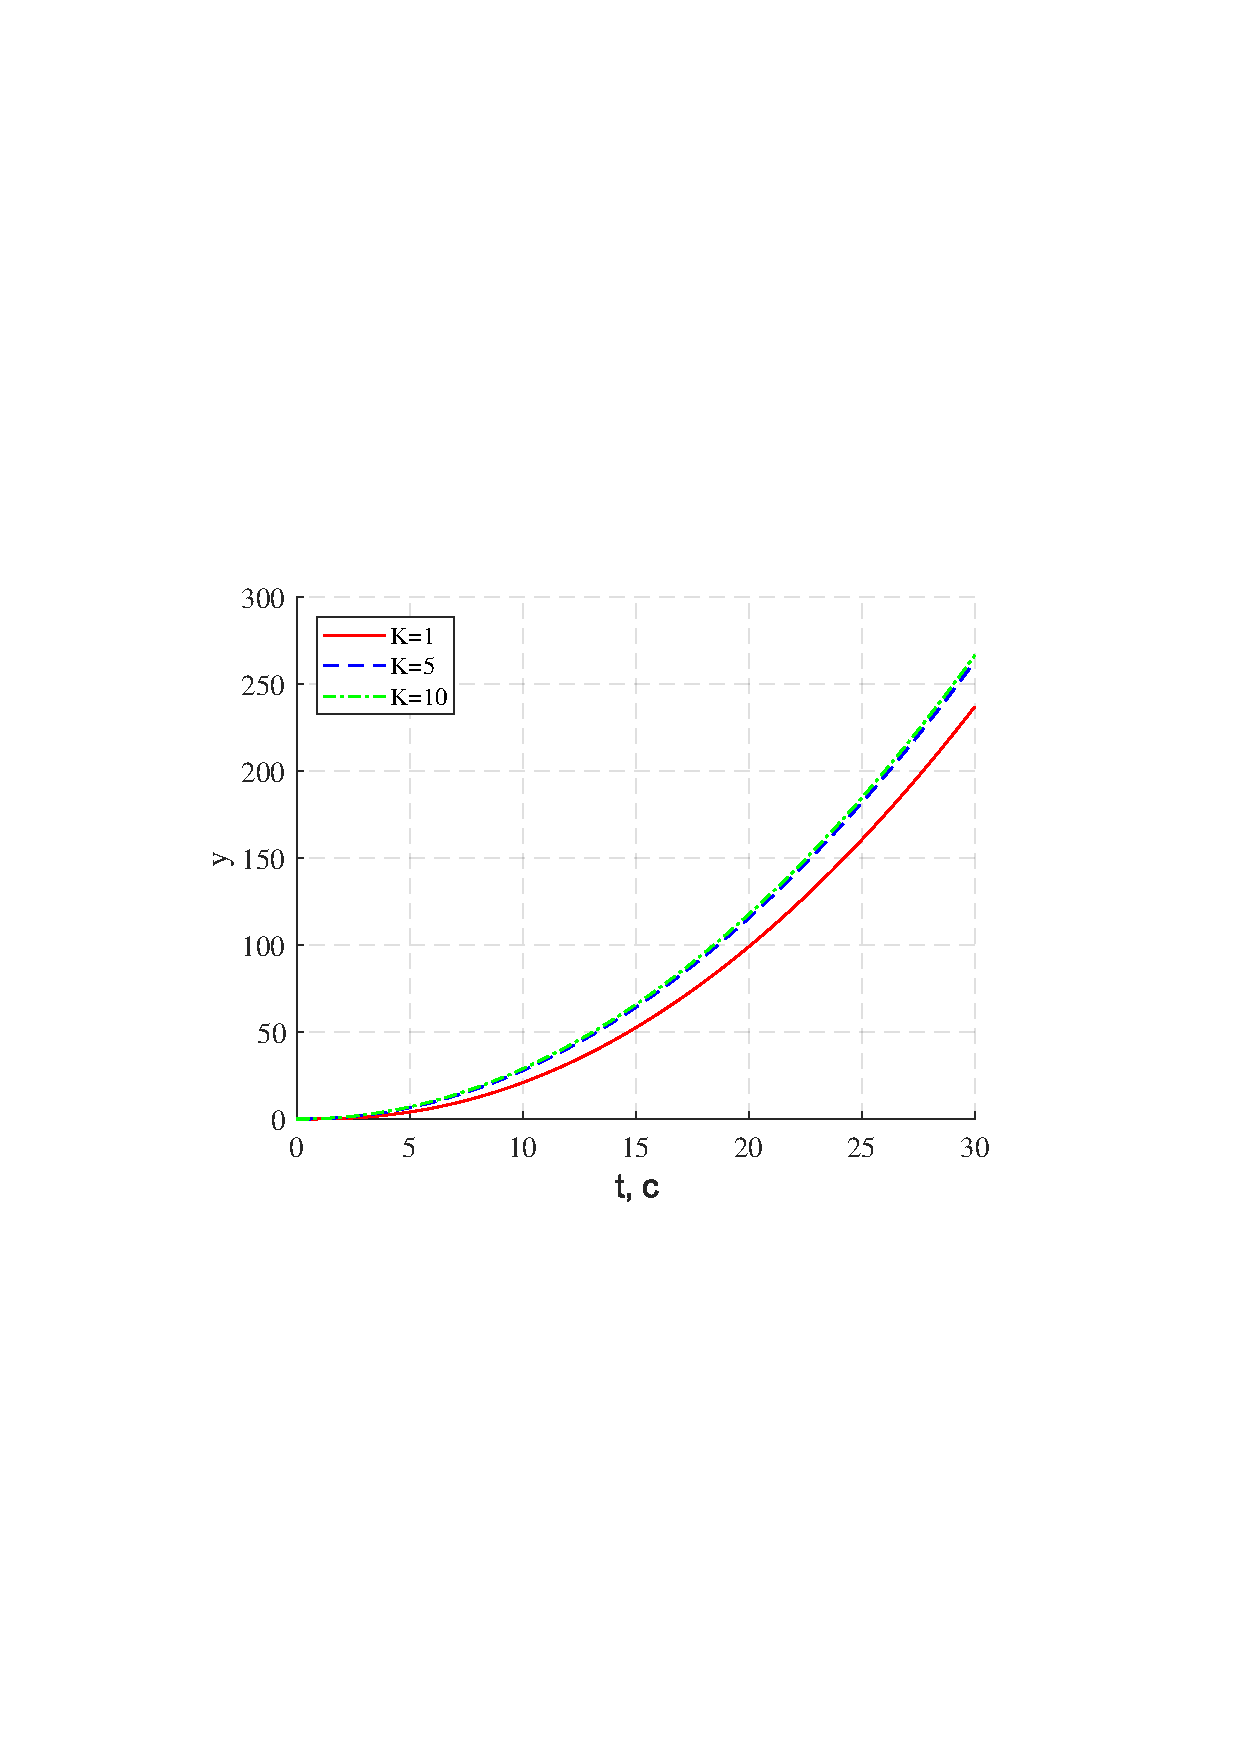
\includegraphics[width=5in]{ph3ast1MOD.pdf}
		\caption{Переходные процессы} 
		\label{s_14} 
		\end{center}
	\end{figure}
	\begin{figure}[h!]
		\begin{center}
		\renewcommand{\figurename}{Рисунок}
		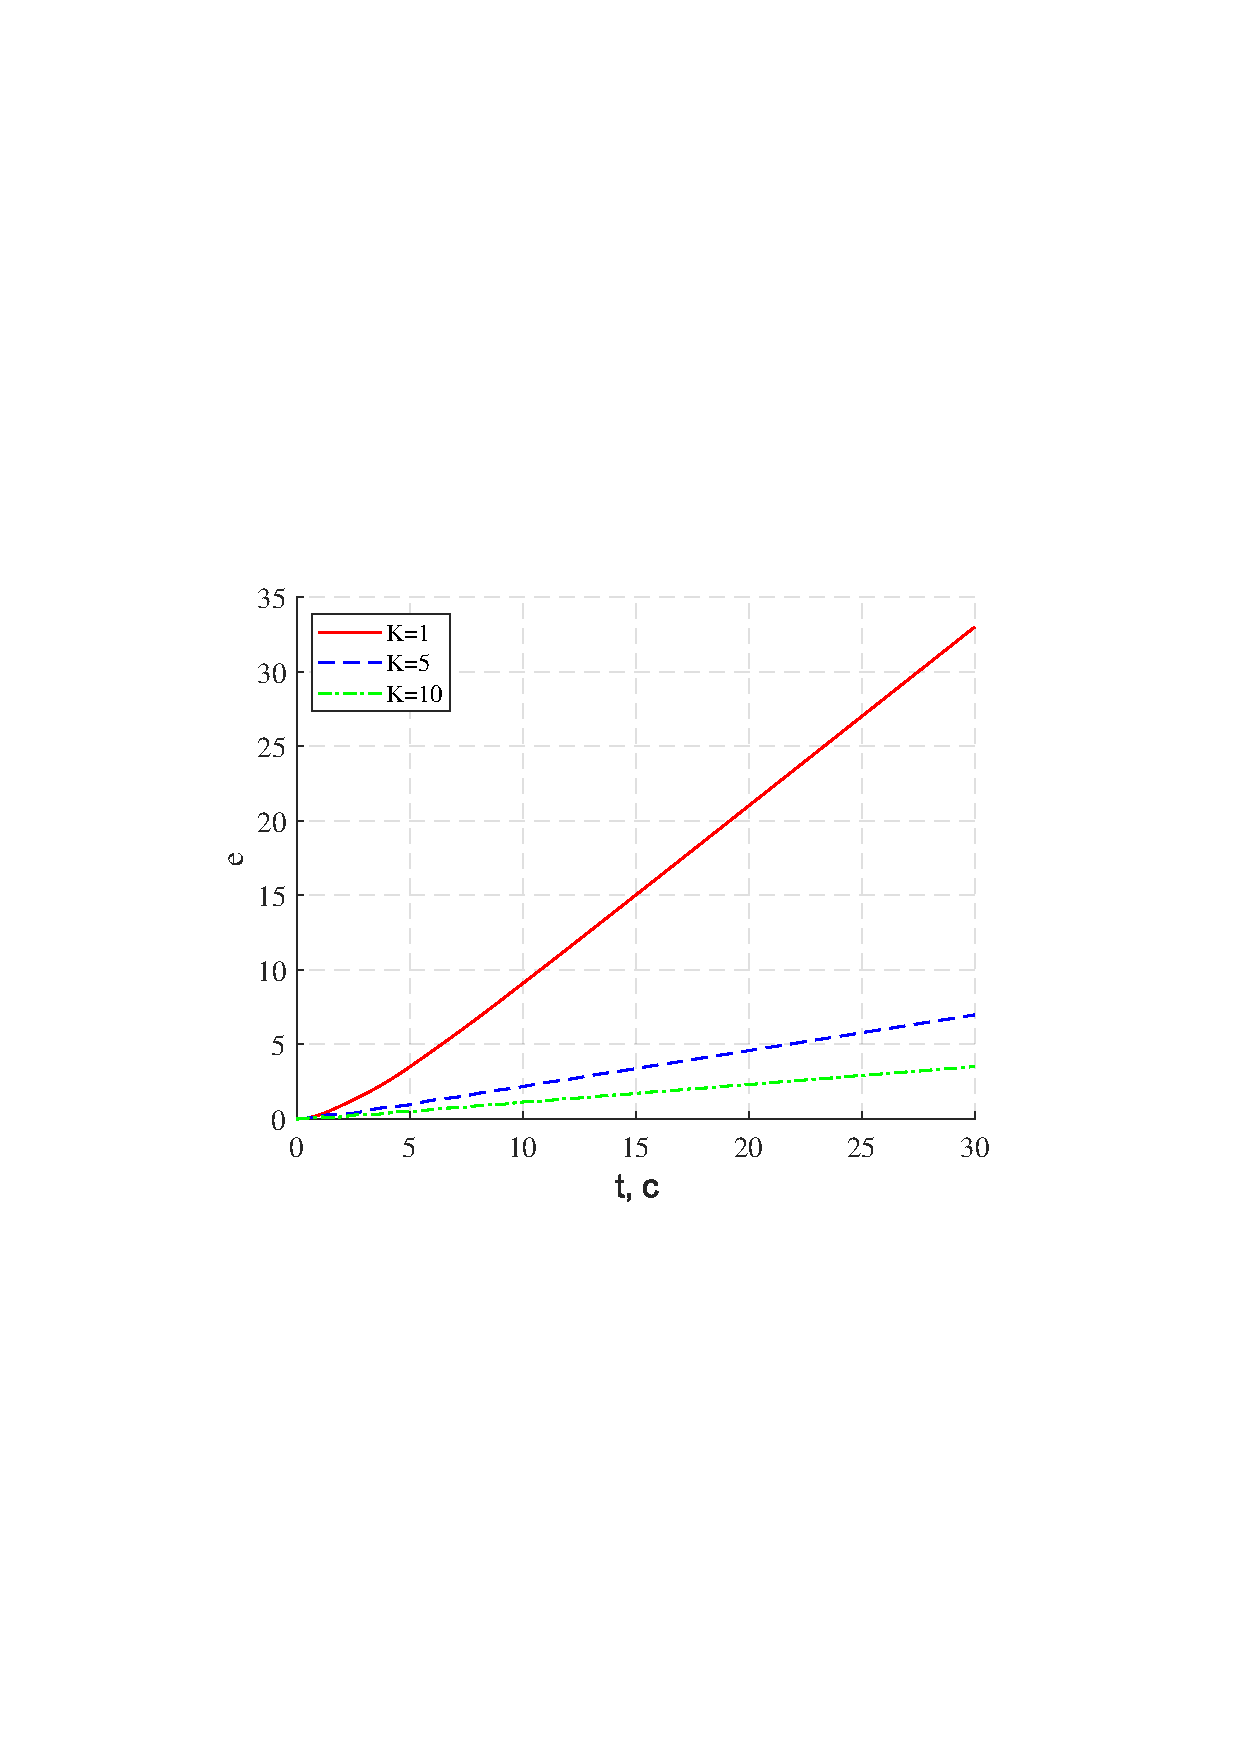
\includegraphics[width=5in]{err3ast1MOD.pdf}
		\caption{Ошибка}
		\label{s_15}
		\end{center}
	\end{figure}
	\newpage
	\begin{center}		
		\section{Исследование влияния внешних возмущений}
	\end{center}
	\paragraph {} Схема моделирования представлена на рисунке \ref{s_16}
	
	\begin{figure}[h]
		\renewcommand{\figurename}{Рисунок}
		\centering
		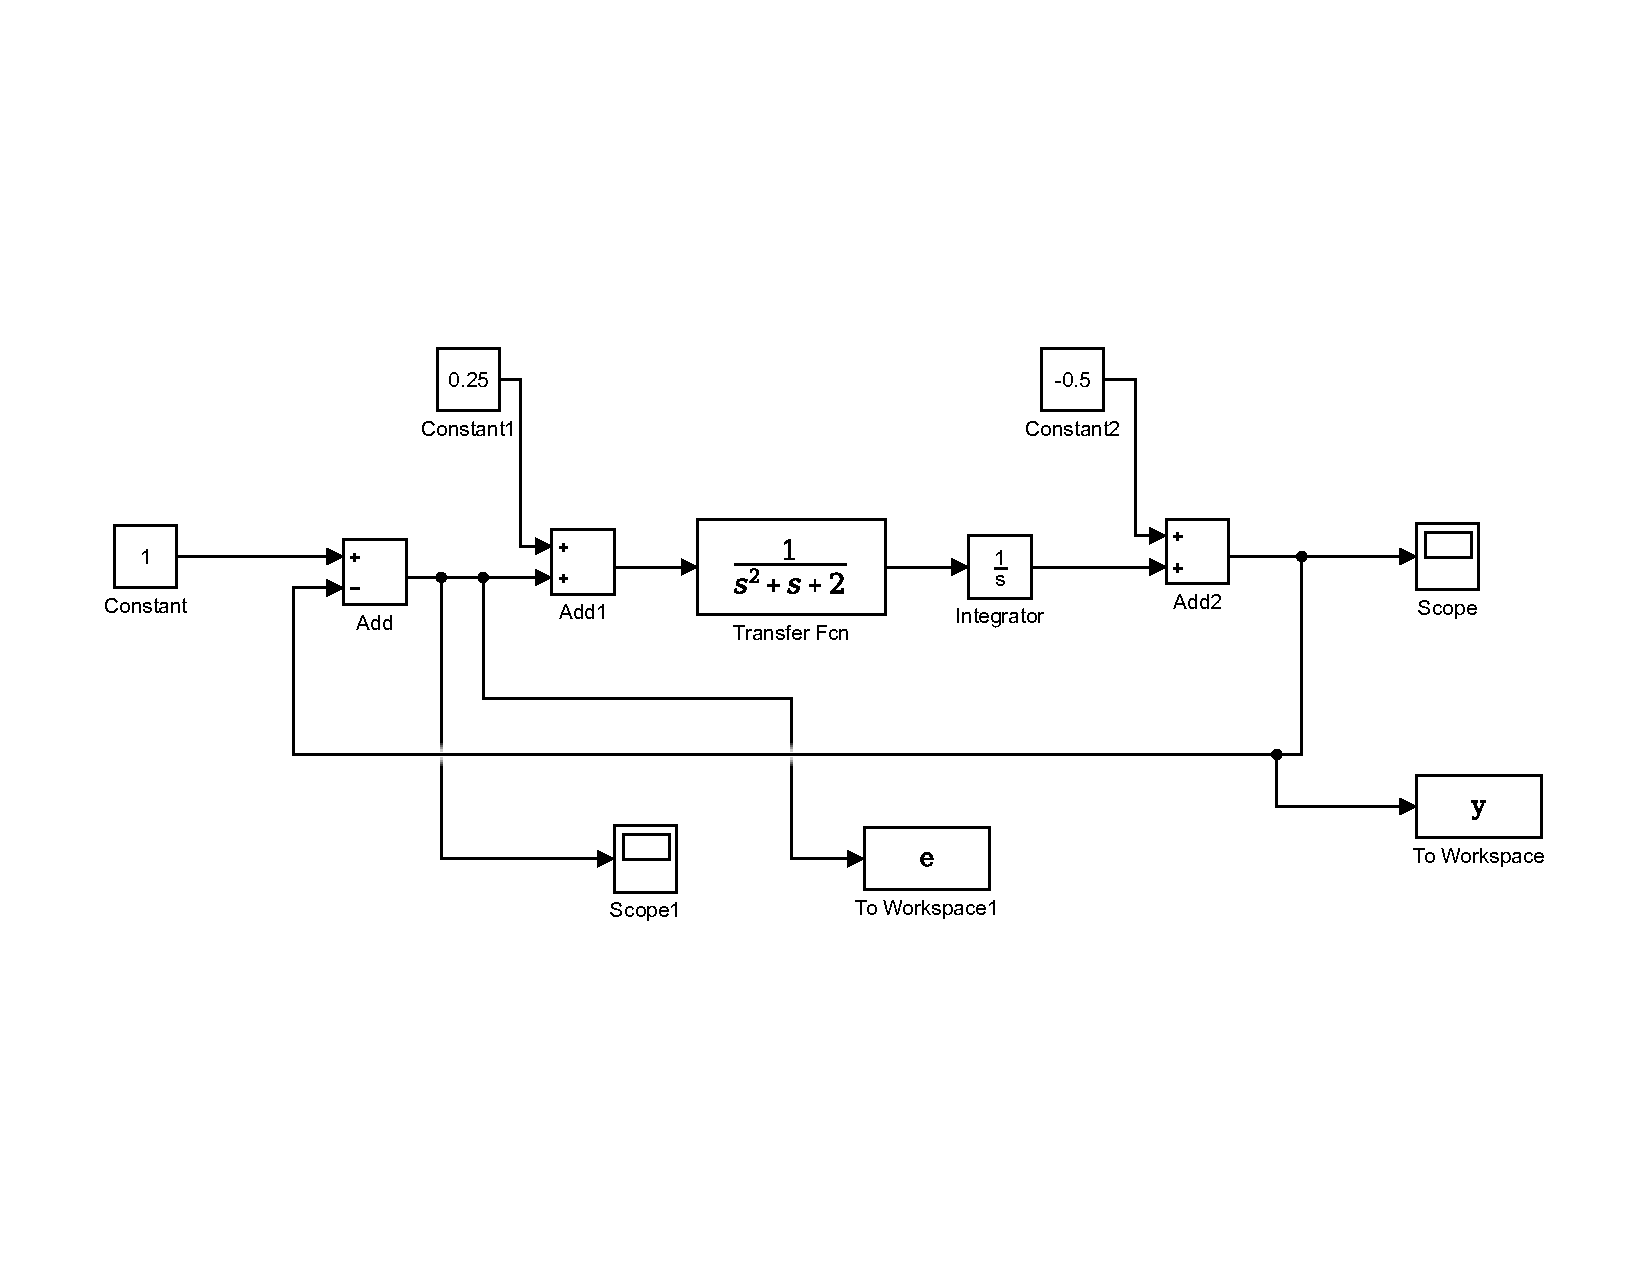
\includegraphics[width=6in]{VozmushenieMOD.pdf}
		\caption{Схема моделирования}
		\label{s_16}
	\end{figure}
	\newpage
	\paragraph {}Переходные процессы и график ошибки при различных значениях $f_1$ и $f_2$ представлены на рисунках \ref{s_17} и \ref{s_18} соответственно
	
	\begin{figure}[h!]
		\begin{center}
		\renewcommand{\figurename}{Рисунок}
		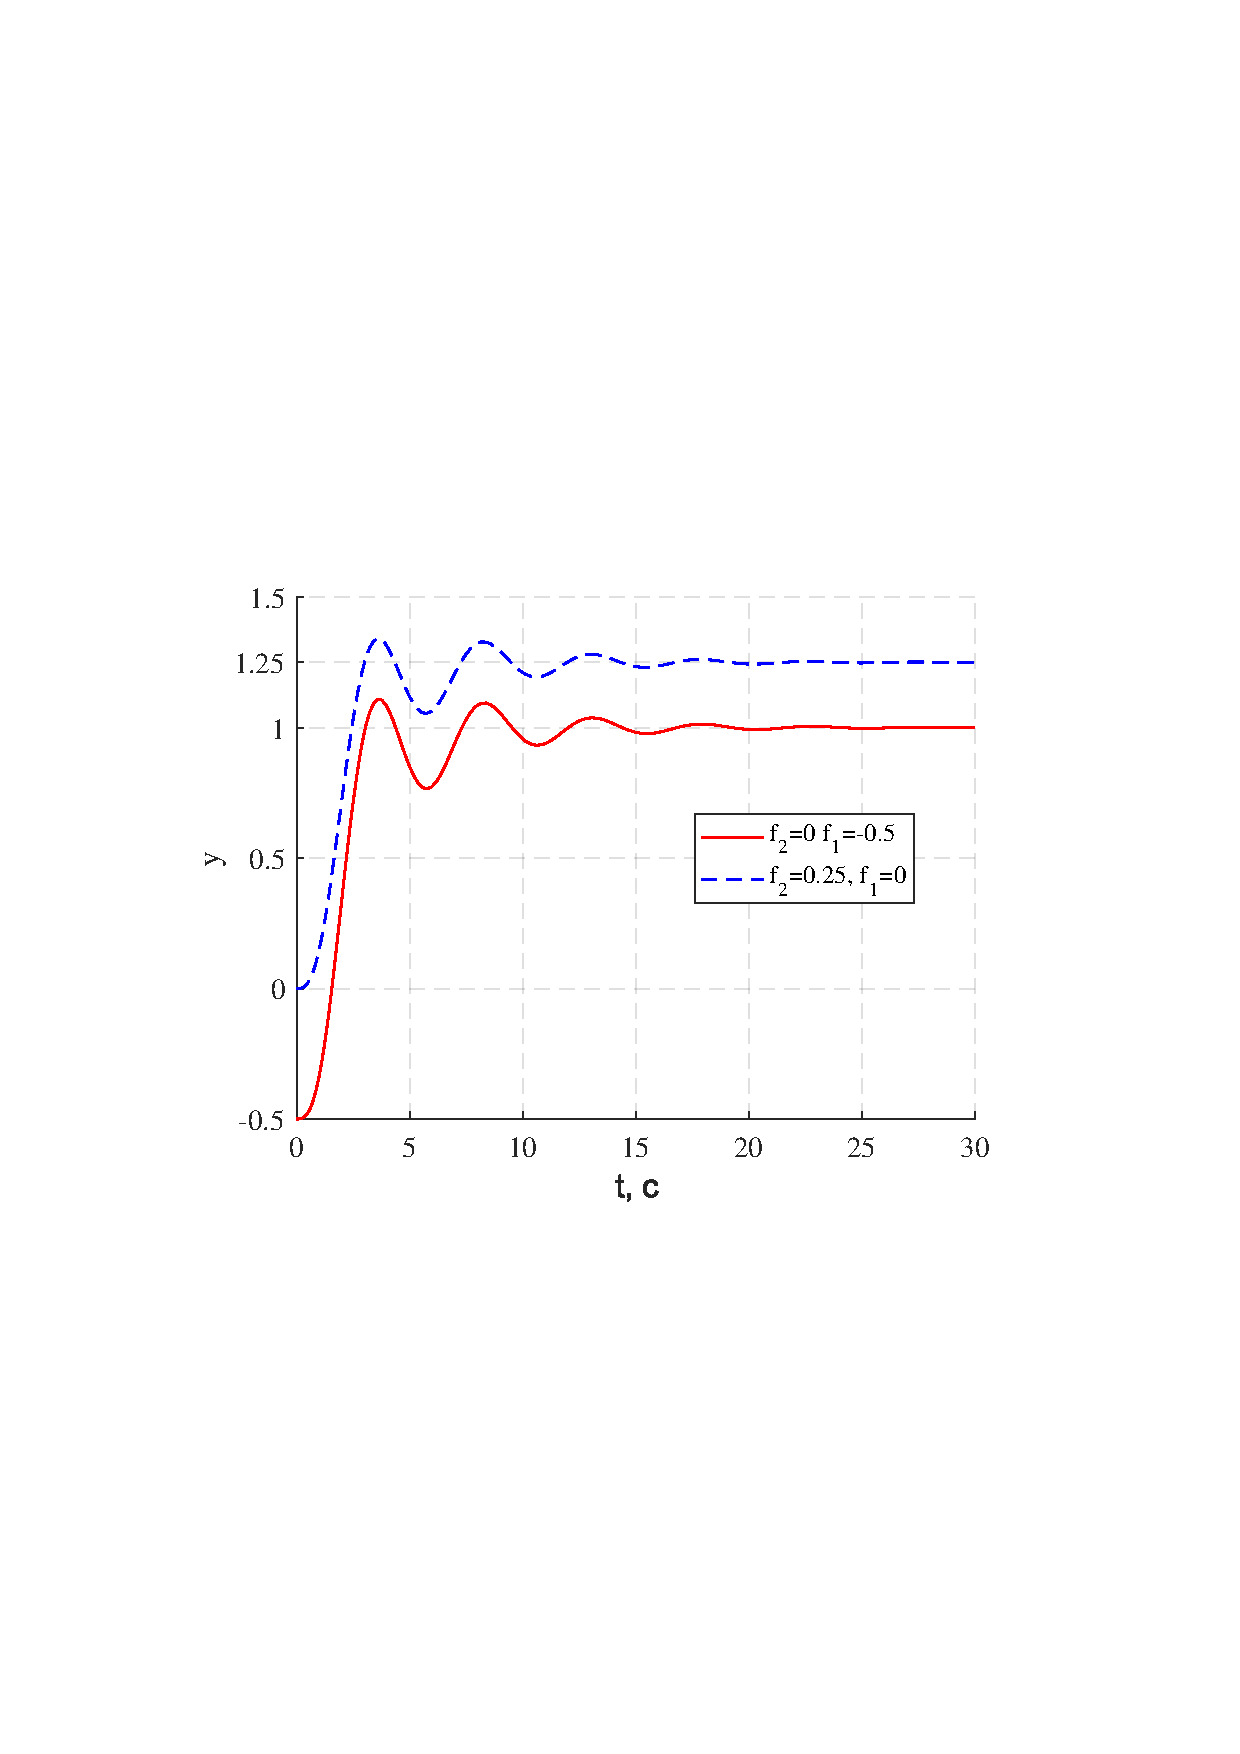
\includegraphics[width=5in]{vozm1MOD.pdf}
		\caption{Переходные процессы} 
		\label{s_17} 
		\end{center}
	\end{figure}
	\begin{figure}[h!]
		\begin{center}
		\renewcommand{\figurename}{Рисунок}
		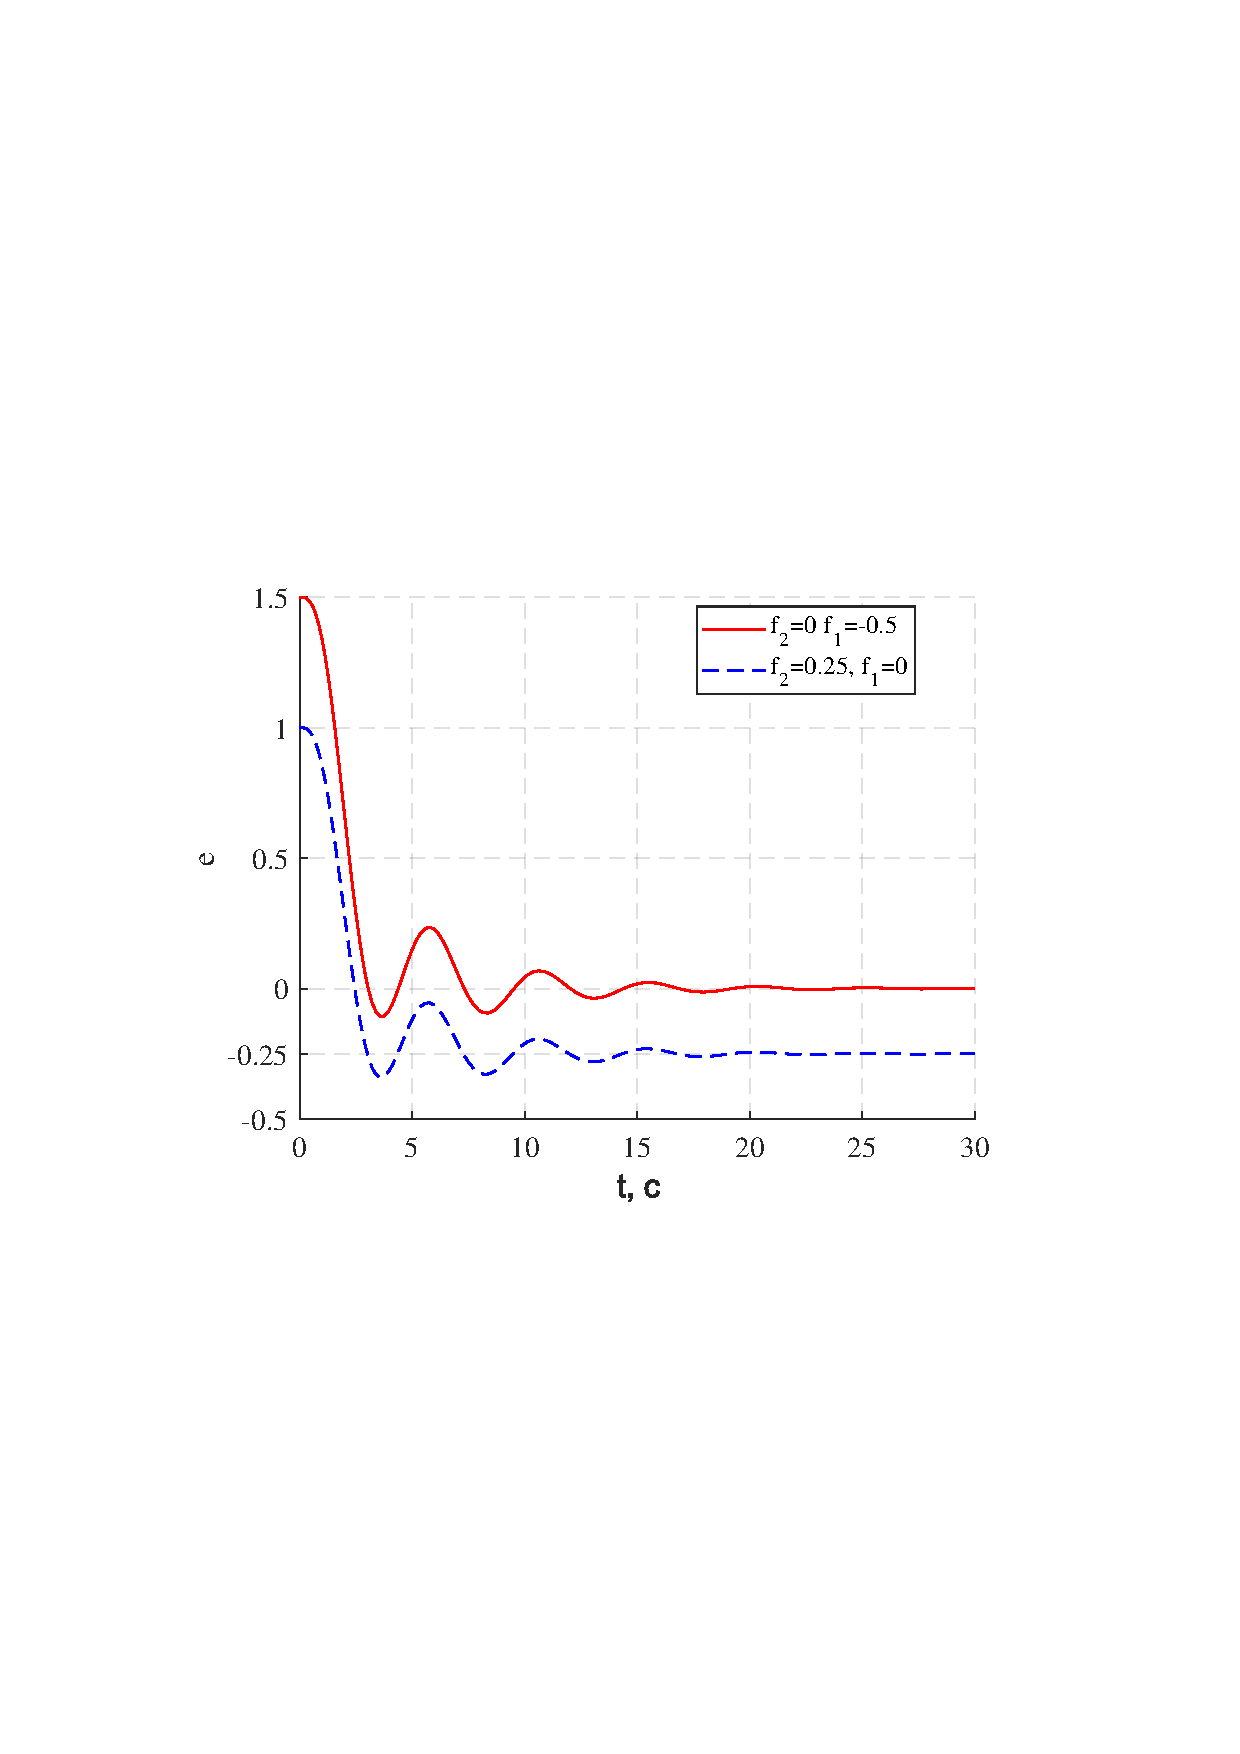
\includegraphics[width=5in]{vozm1errMOD.pdf}
		\caption{Ошибка}
		\label{s_18}
		\end{center}
	
		
	\end{figure}		
	\newpage
	\paragraph {} Аналитический рассчет установившейся ошибки:\\
	\begin{gather}
	\frac{(e+f_2)W(s)}{s}+f_1=y=g-e\\
	e(1+\frac{W(s)}{s})=g-f_1-f_2(\frac{W(s)}{s})\\
	e=\displaystyle \frac{g}{\displaystyle 1+\frac{W(s))}{s}}-\displaystyle\frac{f_1}{\displaystyle 1+\frac{W(s)}{s}}-f_2\frac{W(s)}{s+W(s)}
	\end{gather}
	
	Так как $g$, $f_1$ и $f_2$ постоянные во времени сигналы, то образ Лапласа для каждого из них равен $\frac{g}{s}$, $\frac{f_1}{s}$ и $\frac{f_2}{s}$ соответственно. Отсюда следует, что: \\
	\begin{gather}	 
	\varepsilon=\lim\limits_{s\rightarrow 0}\displaystyle\frac{g}{\displaystyle 1+\frac{W(s))}{s}}-\displaystyle\frac{f_1}{\displaystyle 1+\frac{W(s)}{s}}-f_2\displaystyle\frac{W(s)}{s+W(s)}=-f_2
	\end{gather}
	\begin{itemize}
		\item При $f_2=0$ и $f_1=-0.5$ ~~:~ $\varepsilon=0$
		\item При $f_1=0$ и $f_2=0.25$ ~~:~ $\varepsilon=-0.25$
	\end{itemize}
	\newpage
	\begin{center}
		\section{Исследование установившейся ошибки при произвольном входном воздействии}
	\end{center}
	\paragraph {} Схема моделирования представлена на рисунке \ref{s_19}
	
	\begin{figure}[h]
		\renewcommand{\figurename}{Рисунок}
		\centering
		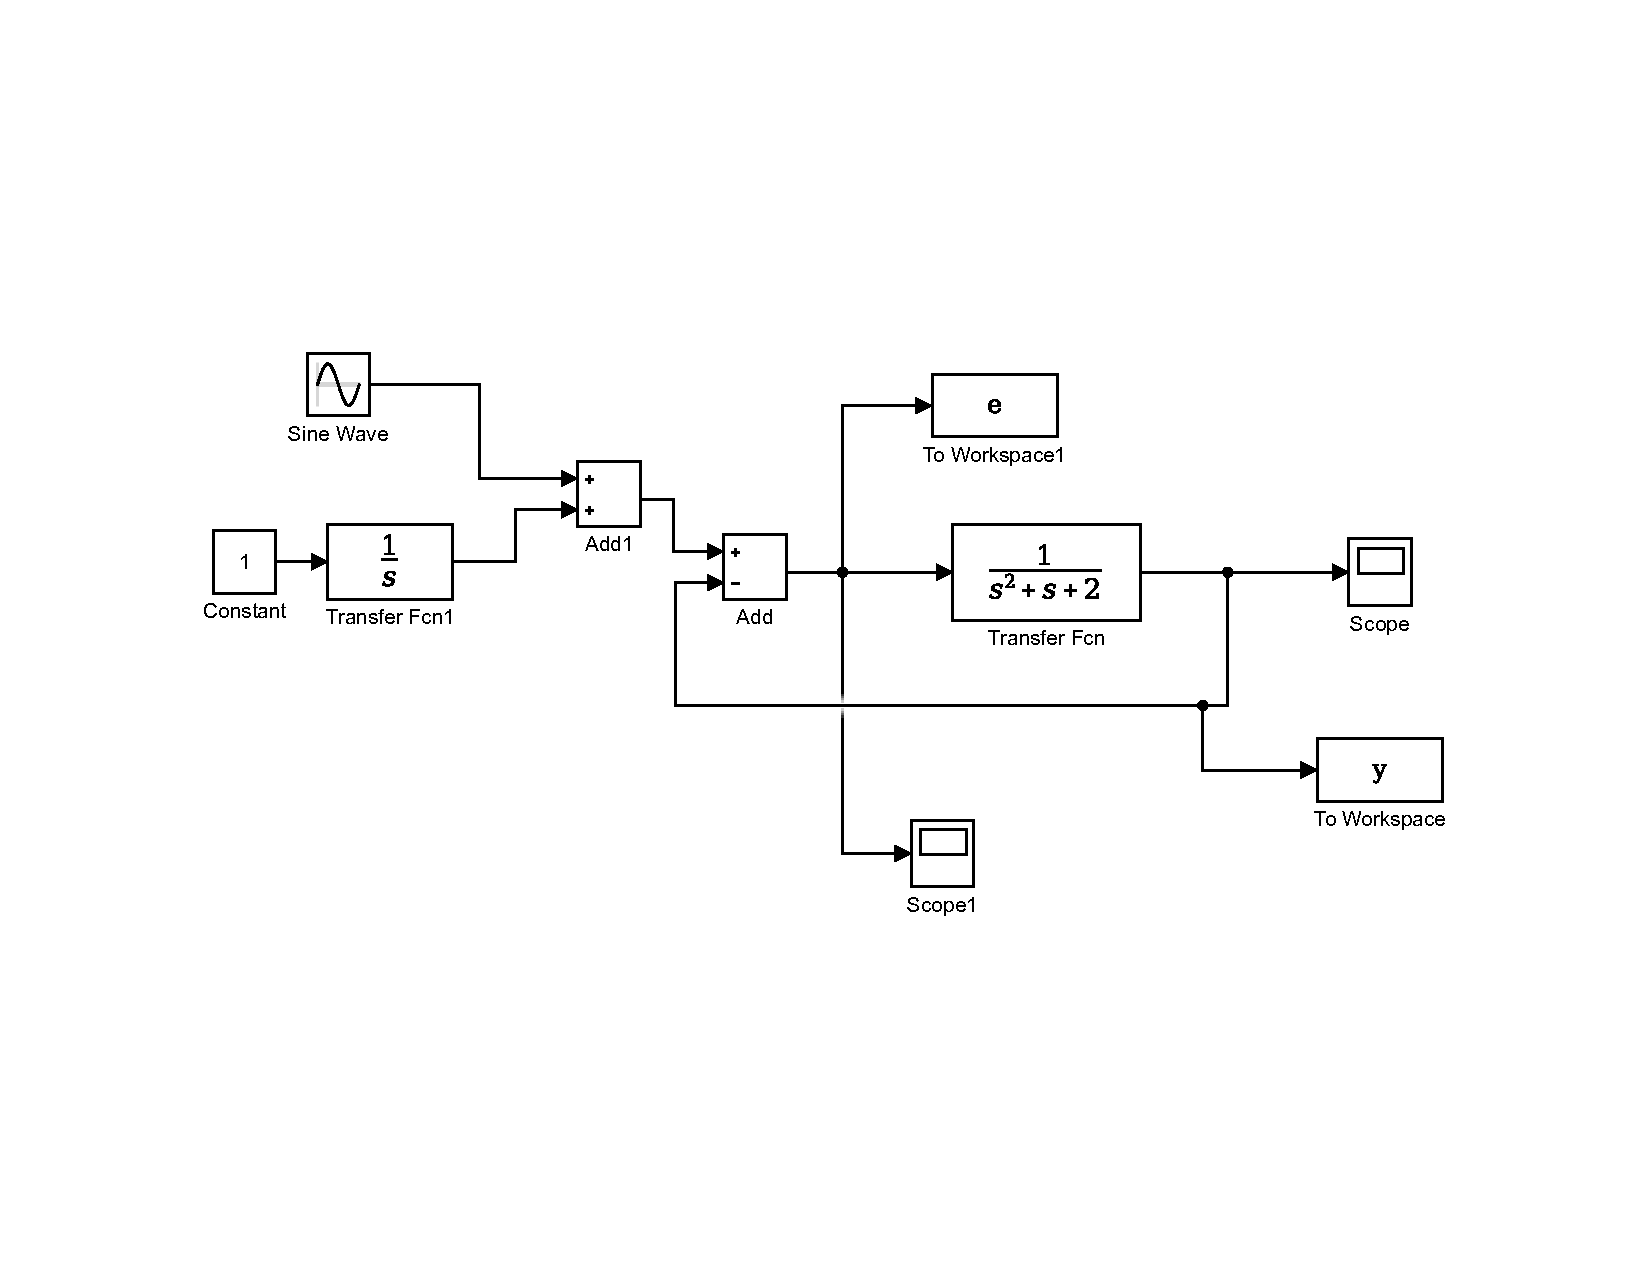
\includegraphics[width=6in]{OshibkaMOD.pdf}
		\caption{Схема моделирования}
		\label{s_19}
	\end{figure}
	\paragraph {}Переходной процесс представлен на рисунке \ref{s_20}
	
	\begin{figure}[h]
		\renewcommand{\figurename}{Рисунок}
		\centering
		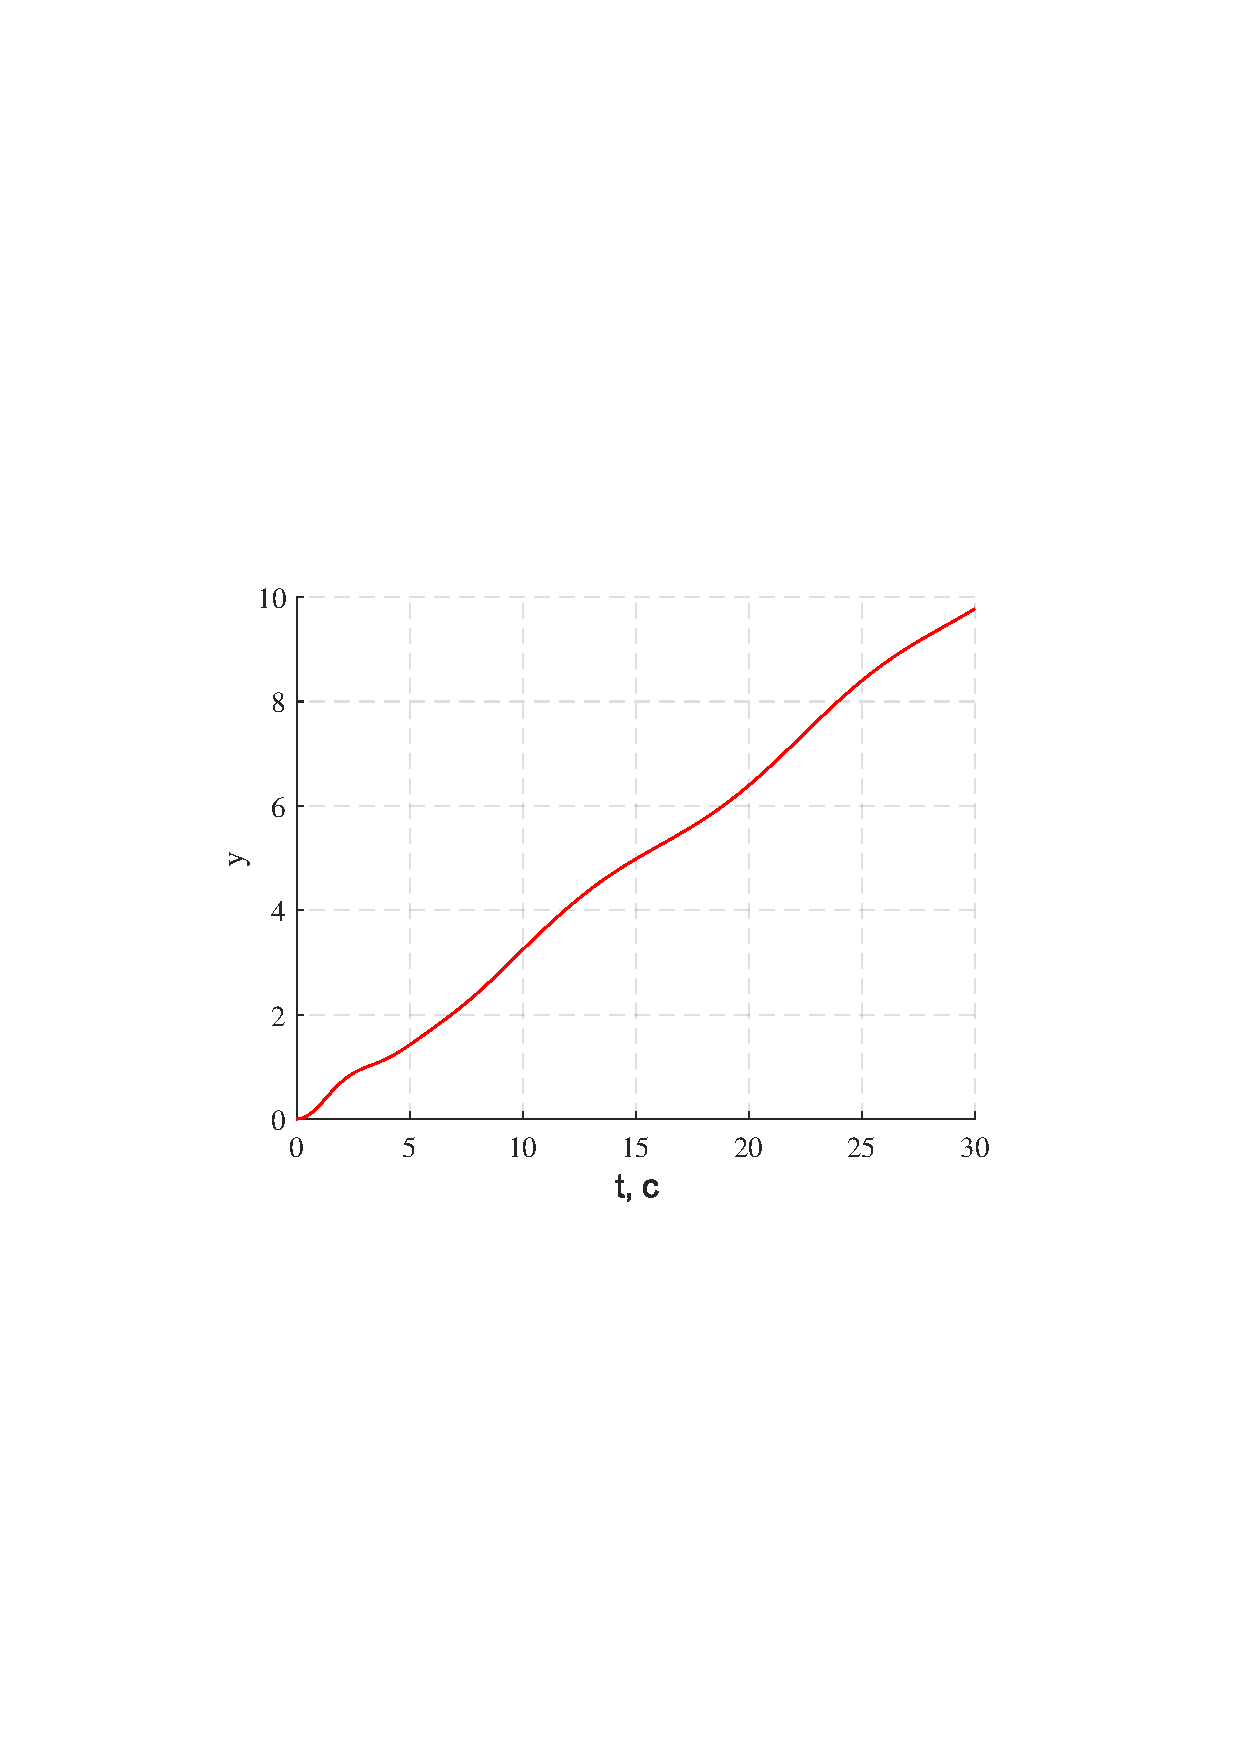
\includegraphics[width=4in]{ph4MOD.pdf}
		\caption{Переходной процесс}
		\label{s_20}
	\end{figure}
	\newpage
	\paragraph {}График ошибки при моделировании и теоретической представлен на рисунке \ref{s_21}
	
	\begin{figure}[h]
		\renewcommand{\figurename}{Рисунок}
		\centering
		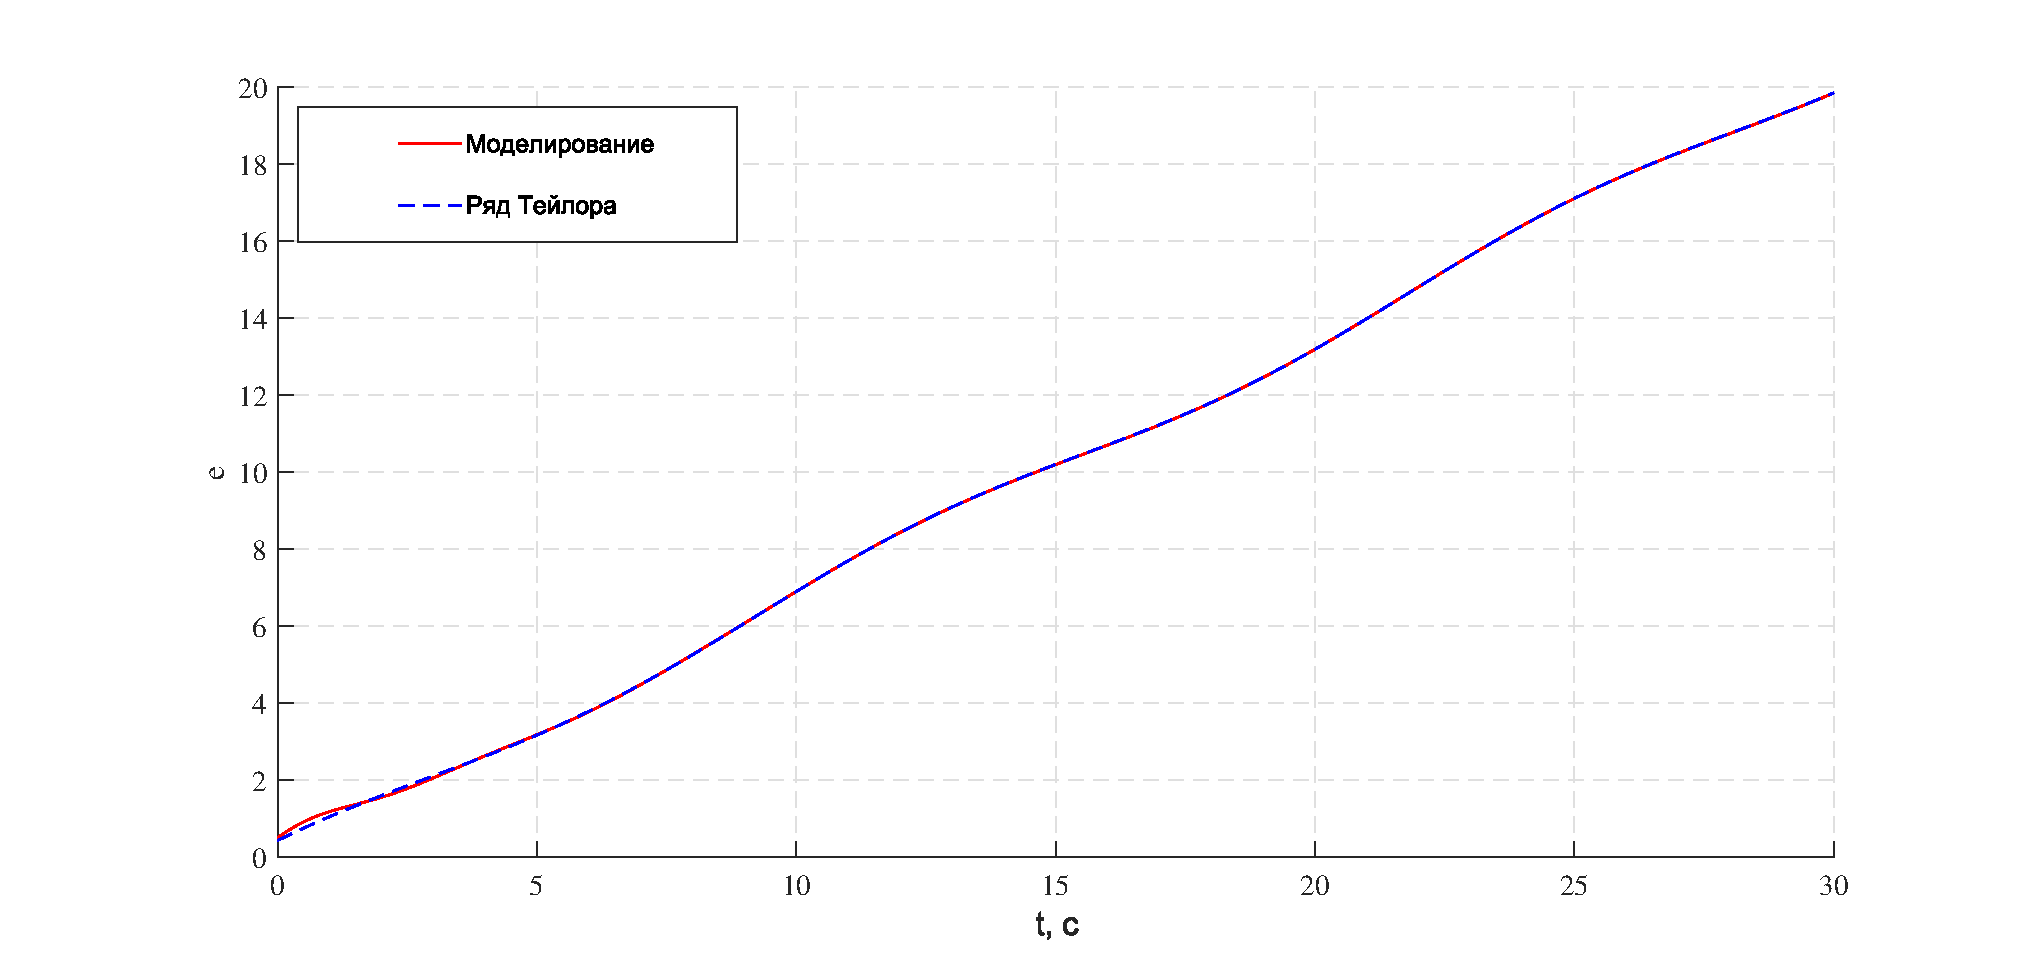
\includegraphics[width=6in]{TailorError.eps}
		\caption{Ошибка}
		\label{s_21}
	\end{figure}
	
	\paragraph {} Приближенное разложение ошибки в ряд Тейлора, содержащий только 3 члена:\\
	\begin{gather}
	E(S)=\Phi_e(s)G(s) ~\text{,~где}~ \displaystyle \Phi_e(s)=\frac{s^2+s+2}{s^2+s+3})\\
	e(t)=c_0g(t)+c_1\dot{g(t)}+c_2\frac{\ddot{g(t)}}{2!}~~\text{, где:}\\
	c_0=\Phi_e(s)_{s=0}=\frac{2}{3}\\
	c_1=(\frac{d\Phi_e(s)}{ds})_{s=0}=\frac{1}{9}\\
	c_2=(\frac{d^2\Phi_e(s)}{ds^2})_{s=0}=\frac{4}{27}\\
	g(t)=t+0.5cos{0.5t}\\
	\dot{g(t)}=1-0.25sin{0.5t}\\
	\ddot{g(t)}=-0.125cos{0.5t}\\
	\end{gather}
	В итоге:
	\begin{gather}
	e(t)=\frac{2}{3}(t+0.5cos{0.5t})+\frac{1}{9}(1-0.25sin{0.5t})+\frac{4}{27}\frac{-0.125cos{0.5t}}{2!}
	\end{gather}
	\newpage
	\begin{center}
		\section*{Вывод}  ~~\\
	\end{center}
	\par
	В данной работе были исследованы две системы с различным порядком астатизма. Для каждой из систем было произведено моделирование при различных входных воздействиях и коэффициентах усиления, в результате которого были получены переходные процессы и установившиеся значения ошибки, которые подтвердились аналитическим расчетом.
	\par Для системы с нулевым порядком астатизма ошибка в стационарном режиме имеет конечное значение, которое уменьшается, при увеличении $k$, а при линейно возрастающем сигнале стремится к бесконечности.
	\par Для системы с первым порядком астатизма значение ошибки в стационарном режиме равно нулю, при линейно возрастающем - имеет некоторое конечное значение, которое уменьшается, при увеличении $k$, а при квадратичном сигнале - стремится к бесконечности.    
	\par Также было исследовано влияние внешних возмущений и аналитический рассчет установившейся ошибки. В результате было выявлено, что для устранения ошибки от постоянного сигнала возмущения необходимо интегрирующий элемент ставить до места приложения этого возмущения.
	\par Было произведено моделирование системы при произвольном входном воздействии. Рассчитанная и полученная при моделировании ошибки совпали. 
	
\end{document}